\section{Lumped-element thermal model of a building}\;abel{s:lumped-element}

Heat generation and transport inside a building, with heat loss to the surrounding outdoor environment is governed by the same laws of conduction, convection and radiation as elsewhere. A number of approximations is made, however, which will be treated below:

\subsection{Heat Conduction: Fourier's Law}

Heat transport \emph{within} a solid material is governed by conduction, according to Fourier's Law, illustrated in Figure \ref{fig:heatcond_1d}.
One side of a rectangular solid is held at temperature $T_1$, while the opposite side is held at a lower temperature, $T_2$. The other four sides are insulated so that heat can flow only in the $x$-direction. For a given material, it is found that the rate, $\dot{Q_x}$ , at which heat (thermal
energy) is transferred from the hot side to the cold side (the \emph{heat transfer rate}) is proportional to the cross-sectional area, $A$, across which the heat flows; the temperature difference, $T_1 - T_2$; and inversely proportional to
the thickness, $\Delta x$, of the material. That is:

\begin{equation}
	\label{eq:fourierlaw}
	\dot{Q_x} = - kA \frac{\Delta T}{\Delta x}
\end{equation}

\begin{figure}[H]
	\centering
	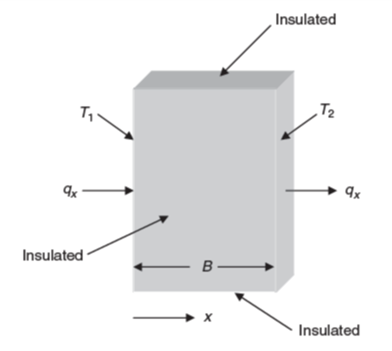
\includegraphics[width=0.5\columnwidth]{Pictures/heat_conduction_1d.png}
	\caption[Short title]{One-dimensional heat conduction in a solid}
	\label{fig:heatcond_1d}
\end{figure} 

The constant of proportionality, $k$, is called the \emph{thermal conductivity}. Equation \eqref{eq:fourierlaw} is also applicable to heat conduction in liquids and gases. However, when temperature differences exist in fluids, convection currents tend to be set up, so that heat is generally not transferred solely by the mechanism of conduction. The thermal conductivity is a property of the material. Values may be found in various handbooks and compendiums of physical property data.

The form of Fourier’s law given by Equation \eqref{eq:fourierlaw} is valid only when the thermal conductivity can be assumed constant. A more general result can be obtained by writing the equation for an element of differential thickness. in the limit as $\Delta x$ approaches zero, $\frac{\Delta T}{\Delta x} \rightarrow \frac{d T}{d x}$. Thus, substituting in Equation \eqref{eq:fourierlaw} gives:

\begin{equation}
	\label{eq:fourierdiff}
	\dot{Q_x} = - kA \frac{d T}{d x}
\end{equation}

Equation \eqref{eq:fourierdiff} is not subject to the restriction of constant $k$. Furthermore, when $k$ is constant, it can be integrated to yield Equation \eqref{eq:fourierlaw}. Hence, Equation \eqref{eq:fourierdiff} is the general one-dimensional form of Fourier’s law. The negative sign is necessary because heat flows in the positive $x$-direction when the temperature decreases in the $x$-direction. Thus, according to the standard sign convention that
$\dot Q_x$ is positive when the heat flow is in the positive $x$-direction, $\dot Q_x$ must be positive when $dT/dx$ is negative. 

\subsubsection{More than one dimension}

It is often convenient to formulate Fourier's Law in the original phrasing: the \emph{heat flux} $ \dot{\varphi}$  is proportional to the \emph{temperature gradient}. We divide \eqref{eq:fourierdiff} by the area to give:

\begin{equation}
	\label{eq:fourierflux}
	\dot{\varphi_x} \equiv \frac{\dot Q_x}{A}- k \frac{d T}{d x}
\end{equation}

where $\dot{\varphi_x}$ is the heat flux. It has units of $\frac{J}{s \cdot m^2} = \frac{W}{m^2}$. 
Thus, the units of $k$ are $\frac{W}{m \cdot K}$.

Equation \eqref{eq:fourierflux} is restricted to the situation in which heat flows in the $x$-direction
only. In the general case in which heat flows in all three coordinate directions, the total heat flux is obtained by vector addition of adding the fluxes in the coordinate directions. Thus,

\begin{equation}
	\label{eq:flux3d}
	\boldsymbol{\dot{\varphi}} = \dot{\varphi_x} \mathbf{i} + \dot{\varphi_y} \mathbf{j} + \dot{\varphi_z} \mathbf{k}
\end{equation}

where $\boldsymbol{\dot{\varphi}}$ is the heat flux vector and \textbf{i}, \textbf{j}, \textbf{k} are unit vectors in the x-, y-, z-directions, respectively.

Each of the component fluxes is given by a one-dimensional Fourier expression as follows:

\begin{equation}
	\begin{aligned}
		\label{eq:fourier3d}
		\dot{\varphi_x} = - k \frac{\partial T}{\partial x} & \qquad & \dot{\varphi_y} = - k \frac{\partial T}{\partial y} & \qquad & \dot{\varphi_z} = - k \frac{\partial T}{\partial z}
	\end{aligned}
\end{equation}

Partial derivatives are used here since the temperature now varies in all three directions. Substituting
the above expressions for the fluxes into Equation \eqref{eq:flux3d} gives:

\begin{equation}
	\label{eq:fouriercart}
	\boldsymbol{\dot{\varphi}} = -k \left(\frac{\partial T}{\partial x} \mathbf{i} + \frac{\partial T}{\partial y} \mathbf{j} + \frac{\partial T}{\partial z} \mathbf{k} \right)
\end{equation}

The vector in parenthesis is the temperature gradient vector, and is denoted by $\nabla T$. Hence,

\begin{equation}
	\label{eq:fouriernabla}
	\boldsymbol{\dot{\varphi}} = -k \nabla T
\end{equation}

Equation \eqref{eq:fouriernabla} is the three-dimensional form of Fourier’s law. It is valid for homogeneous, isotropic materials for which the thermal conductivity is the same in all directions. Fourier’s law states that heat flows in the direction of greatest temperature decrease.

\subsubsection{The Heat Conduction Equation}

The solution of problems involving heat conduction in solids can, in principle, be reduced to the
solution of a single differential equation, the \emph{heat conduction equation}. The equation can be derived
by making a thermal power balance on a differential volume element in the solid. For the case of
conduction in the $x$-direction only, such a volume element is illustrated in Figure \ref{fig:element_1d}. 

\begin{figure}[H]
	\centering
	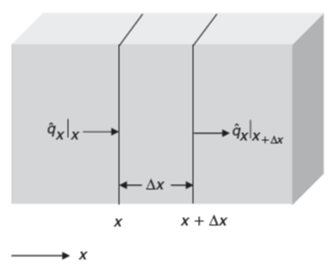
\includegraphics[width=0.5\columnwidth]{Pictures/Element.png}
	\caption[Short title]{Differential element for 1D heat conduction}
	\label{fig:element_1d}
\end{figure}

The rate at which thermal energy enters the volume element across the face at $x$ is given by the
product of the heat flux and the cross-sectional area, $\dot{\varphi_x}|_x \cdot A$.
Similarly, the rate at which thermal energy leaves the element across the face at $x + \Delta x$ is $\dot{\varphi_x}|_{x + \Delta x} \cdot A$. 

A heat generation term appears in the equation because the balance is made on thermal energy, not
total energy. For example, thermal energy may be generated within a solid by an electric current
or by decay of a radioactive material.

For a homogeneous heat source of strength $\dot{q}$ \emph{per unit volume}, the net rate of generation is $\dot{q}A \Delta x$. Finally, the rate of accumulation of heat in the material is given by the time derivative of the thermal energy content of the volume element, which is $\rho c(T - T_{ref} )A\Delta x$, where $T_{ref}$ is an arbitrary reference temperature. Thus, the balance equation
becomes:

\begin{equation}
	\label{eq;heatbalance}
	\left( \dot{\varphi_x}|_x - \dot{\varphi_x}|_{x + \Delta x} \right)A + \dot{q}A \Delta x = \rho c  \frac{\partial T}{\partial t}A\Delta x
\end{equation}

It has been assumed here that the density, $\rho$, and heat capacity, $c$, are constant. 

Dividing by $A \Delta x$ and taking the limit as $\Delta x \rightarrow 0 $ yields:

\begin{equation}
	\rho c  \frac{\partial T}{\partial t} = -\frac{\partial \dot{\varphi_x}}{\partial x} + \dot{q}
\end{equation}

Using Fourier’s law as given by Equation \eqref{eq:fourierflux}, the balance equation becomes:

\begin{equation}
	\rho c  \frac{\partial T}{\partial t} = \frac{\partial}{\partial x} \left(\frac{k \partial T}{\partial x} \right)+ \dot{q}
\end{equation}

When conduction occurs in all three coordinate directions, the balance equation contains y- and
z-derivatives analogous to the x-derivative. The balance equation then becomes:

\begin{equation}
	\label{eq:heat3d}
	\rho c  \frac{\partial T}{\partial x} = \frac{\partial}{\partial x} \left(\frac{k \partial T}{\partial x} \right)  + \frac{\partial}{\partial y} \left(\frac{k \partial T}{\partial y} \right) + \frac{\partial}{\partial z} \left(\frac{k \partial T}{\partial z} \right) + \dot{q}
\end{equation}

When $k$ is constant, it can be taken outside the derivatives and Equation \eqref{eq:heat3d} can be written as:	

\begin{equation}
	\frac{\rho c}{k}  \frac{\partial T}{\partial t} = \frac{\partial^2 T}{\partial x^2}  + \frac{\partial^2 T}{\partial y^2} + \frac{\partial^2 T}{\partial z^2} + \frac{\dot{q}}{k}
\end{equation}

or

\begin{equation}
	\frac{1}{\alpha} \frac{\partial T}{\partial t} = \nabla^2 T + \frac{\dot{q}}{k}
\end{equation}

where $\alpha \equiv k /\rho c$ is the \emph{thermal diffusivity} and $\nabla^2$ is the Laplacian operator. The thermal diffusivity has units of $m^2/s$.


\subsection{Convection: Newton's Law of cooling}

When a solid is \emph{immersed} in a fluid or atmospheric gas, heat transfer on the interface occurs by convection. This phenomenon is governed by Newton's Law of cooling:

“The rate of heat lost by a body is directly proportional to the temperature difference of a body and its surroundings”

\begin{equation}
	\label{eq:newtonlaw}
	\dot{Q_x} = - hA \Delta T
\end{equation}

\subsection{Radiation}

\subsection{Approximations: A Simplified Model}

In building physics, it is often assumed that Fourier's Law is valid in the form of Eq. \eqref{eq:fourierlaw}. This can be done under the condition that 

\begin{equation}
	\begin{aligned}
	    \nabla^2 T \equiv 0 & \rightarrow & \frac{\partial T}{\partial \mathbf{r}} = constant
    \end{aligned}
\end{equation}

\subsection{Lumped-element matrix representation}

We take the 2R-2C lumped-element model from Section 2:

\begin{figure}[H]
	\centering
	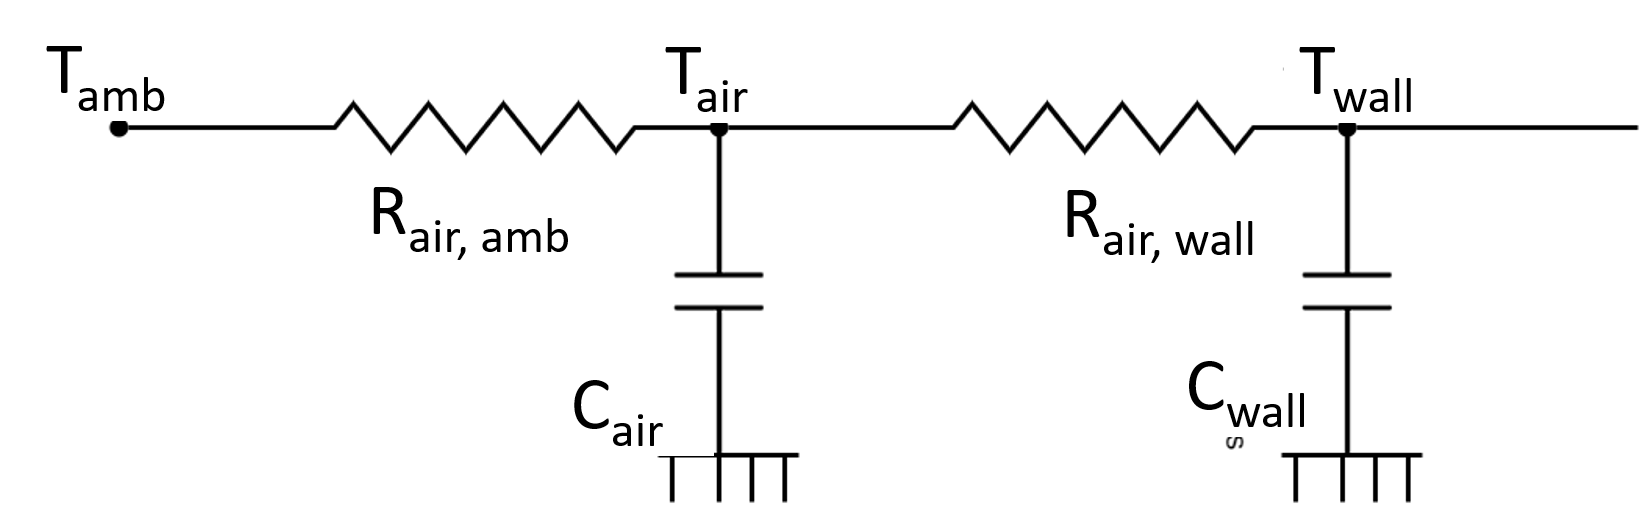
\includegraphics[width=0.7\columnwidth]{Pictures/2R2Cmodel_rev.png}
	\caption[Short title]{2R-2C house model revisited}
	\label{fig:elec2R2Cbis}
\end{figure}

The differential equations are:

\begin{equation}
	\begin{aligned}
	C_{air}\frac{dT_{air}}{dt} &=\frac{T_{amb}-T_{air}}{R_{air, amb}} + \frac{T_{wall}-T_{air}}{R_{air, wall}} + \dot{Q}_{heat, air} + \dot{Q}_{int, air} + \dot{Q}_{solar, air} 
	\\ \\
	C_{wall}\frac{dT_{wall}}{dt} &=\frac{T_{air}-T_{wall}}{R_{air, wall}} + \dot{Q}_{solar, wall}
    \end{aligned}
\end{equation}

Writing out the differential equations in the classical notation:

\begin{equation}
	\begin{aligned}
		C_{air}\frac{dT_{air}}{dt} &= \left[ \frac{-1}{R_{air, amb}} + \frac{-1}{R_{air, wall}} \right]  \cdot T_{air}  + \frac{1}{R_{air, wall}} \cdot T_{wall} + \frac{1}{R_{air, amb}} \cdot T_{amb} + \dot{Q}_{heat, air} + \dot{Q}_{int, air} + \dot{Q}_{solar, air} 
		\\ \\
		C_{wall}\frac{dT_{wall}}{dt} &= \frac{1}{R_{air, wall}} \cdot T_{air} + \frac{-1}{R_{air, wall}}   \cdot T_{wall} + \dot{Q}_{solar, wall}
	\end{aligned}
\end{equation}

The differential equations can be written in matrix notation as:

\begin{subequations}
	\label{eq:matnot}
	\begin{align}
	\mathbf{C} \cdot \boldsymbol{\dot{\theta}} = - \mathbf{K} \cdot \boldsymbol{\theta} + \mathbf{\dot{q}} \\ 
	\mathbf{C} \cdot \boldsymbol{\dot{\theta}} + \mathbf{K} \cdot \boldsymbol{\theta} = \mathbf{\dot{q}}
	\end{align}
\end{subequations}

with:

\begin{equation}
	\mathbf{C} \cdot \boldsymbol{\dot{\theta}} =
	\begin{bmatrix}
		C_{air} & 0 \\
		0 &  C_{wall}
	\end{bmatrix}
    \cdot
    \begin{bmatrix}
    	\frac{dT_{air}}{dt} \\
    	\frac{dT_{wall}}{dt}
    \end{bmatrix}
\end{equation}

\begin{equation}
	\mathbf{K} \cdot \boldsymbol{\theta} =
	\begin{bmatrix}
		\frac{1}{R_{air, amb}} + \frac{1}{R_{air, wall}} & \frac{-1}{R_{air, wall}} \\
		\frac{-1}{R_{air, wall}} &  \frac{1}{R_{air, wall}}
	\end{bmatrix}
	\cdot
	\begin{bmatrix}
		T_{air} \\
		T_{wall}
	\end{bmatrix}
\end{equation}

\begin{equation}
	\mathbf{\dot{q}} =
	\begin{bmatrix}
		\frac{1}{R_{air, amb}} \cdot T_{amb} + \dot{Q}_{heat, air} + \dot{Q}_{int, air} + \dot{Q}_{solar, air} \\
		\dot{Q}_{solar, wall}
	\end{bmatrix}
\end{equation}

Written out, the differential equation according to \eqref{eq:matnot} becomes:

\begin{equation}
	\begin{aligned}
		\begin{bmatrix}
			C_{air} & 0 \\
			0 &  C_{wall}
		\end{bmatrix}
		\cdot
		\begin{bmatrix}
			\frac{dT_{air}}{dt} \\
			\frac{dT_{wall}}{dt}
		\end{bmatrix}
		=
		\begin{bmatrix}
			\frac{-1}{R_{air, amb}} + \frac{-1}{R_{air, wall}} & \frac{1}{R_{air, wall}} \\
			\frac{1}{R_{air, wall}} &  \frac{-1}{R_{air, wall}}
		\end{bmatrix}
		\cdot
		\begin{bmatrix}
			T_{air} \\
			T_{wall}
		\end{bmatrix}
		+ \\ \\
		\begin{bmatrix}
			\frac{1}{R_{air, amb}} \cdot T_{amb} + \dot{Q}_{heat, air} + \dot{Q}_{int, air} + \dot{Q}_{solar, air} \\
			\dot{Q}_{solar, wall}
		\end{bmatrix}
	\end{aligned}
\end{equation}

In the alternative notation:

\begin{equation}
	\begin{aligned}
	\begin{bmatrix}
	    C_{air} & 0 \\
	    0 &  C_{wall}
    \end{bmatrix}
    \cdot
    \begin{bmatrix}
    	\frac{dT_{air}}{dt} \\
    	\frac{dT_{wall}}{dt}
    \end{bmatrix}
    +
    	\begin{bmatrix}
    	\frac{1}{R_{air, amb}} + \frac{1}{R_{air, wall}} & \frac{-1}{R_{air, wall}} \\
    	\frac{-1}{R_{air, wall}} &  \frac{1}{R_{air, wall}}
    \end{bmatrix}
    \cdot
    \begin{bmatrix}
    	T_{air} \\
    	T_{wall}
    \end{bmatrix}
    = \\ \\
    \begin{bmatrix}
        \frac{1}{R_{air, amb}} \cdot T_{amb} + \dot{Q}_{heat, air} + \dot{Q}_{int, air} + \dot{Q}_{solar, air} \\
    	\dot{Q}_{solar, wall}
    \end{bmatrix}
	\end{aligned}
\end{equation}

The lumped-element equations above are systems of \emph{first-order ordinary differential equations} (ODE). The first order derivative is with respect to \emph{time}. The (silent) assumption that heat conduction within the air and the wall of the previous 2R-2C model is \emph{faster} than the exchange of heat at the \emph{interfaces} between air and wall and air and ambient surroundings has replaced all spatial information from the \emph{second-order partial differential equations} (PDE) that govern conductive heat transport \emph{within} materials.

Therefore, the lumped-element equations can be solved by:
\begin{itemize}
	\item the \textsf{odexxx} in Matlab., preferrably \textsf{ode45}.
	\item the \textsf{state-space} module in Simulink, after conversion to a state-space representation.
	\item the \textsf{scipy.integrate.solve\_ivp} function in Python. In older code, \textsf{scipy.integrate.odeint} is still encountered.
	\item in C++ several options exist, similar to the options in Python.
\end{itemize}

The routines in Matlab, Simulink and Python need a \emph{model function} that provides the vector $\boldsymbol{\dot{\theta}}$ for evaluation at any time instance chosen by the algorithm. The equations \eqref{eq:matnot} then should be cast in the following form by left multiplication with $\mathbf{C^{-1}}$.

\begin{subequations}
	\label{eq:matnot_ivp}
	\begin{align}
		\mathbf{C}^{-1} \cdot \mathbf{C} \cdot \boldsymbol{\dot{\theta}} = - \mathbf{C}^{-1} \cdot \mathbf{K} \cdot \boldsymbol{\theta} + \mathbf{C}^{-1} \cdot \mathbf{\dot{q}} \\ 
        \boldsymbol{\dot{\theta}} = - \mathbf{C}^{-1} \cdot \mathbf{K} \cdot \boldsymbol{\theta} + \mathbf{C}^{-1} \cdot \mathbf{\dot{q}}
	\end{align}
\end{subequations}

Since $\mathbf{C}$ is a \emph{diagonal} matrix with positive elements only, its inverse exists and contains the reciprocal elements on its diagonal:

\begin{equation}
	\mathbf{C^{-1}} =
	\begin{bmatrix}
		\frac{1}{C_{air}} & 0 \\
		0 &  \frac{1}{C_{wall}}
	\end{bmatrix}
\end{equation}

This provides the division by the lumped thermal capacitances of the air and wall compartments in the model, necessary for the calculating the derivative vector $\boldsymbol{\dot{\theta}}$ in the model functions. 

\subsection{Extension of the method to larger lumped-element networks}

Take a house model with two stories. Each level in the building is described with a 2R-2C model. Heat transfer occurs between the ground floor and the 1st floor.

\begin{figure}[H]
	\centering
	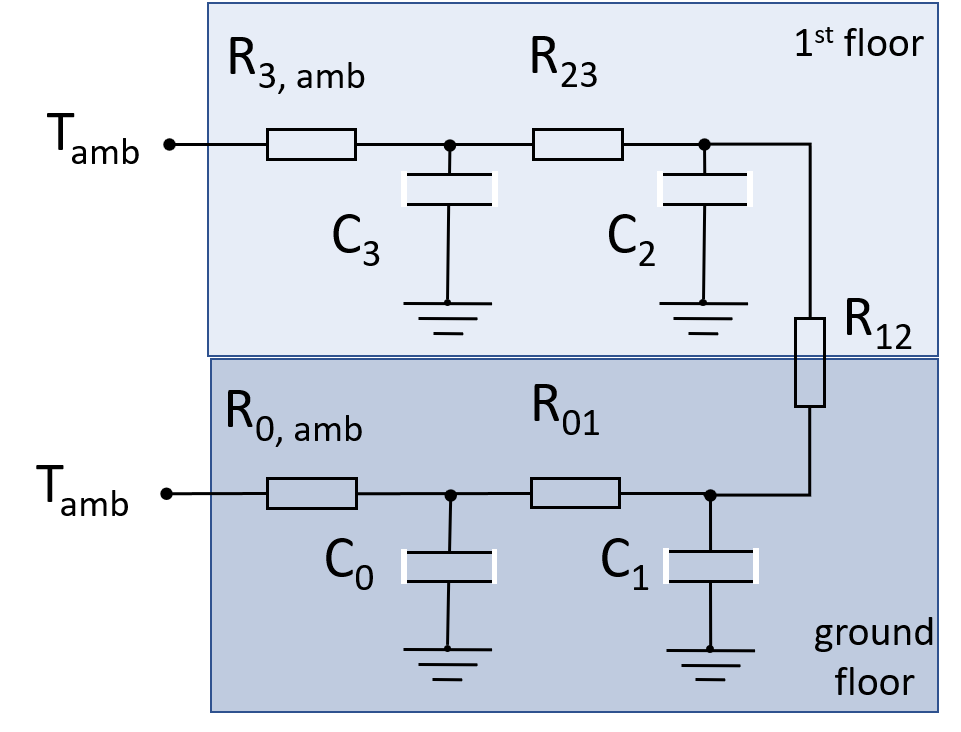
\includegraphics[width=0.6\columnwidth]{Pictures/5R4C.png}
	\caption[Short title]{5R-4C house model}
	\label{fig:elec4R5C}
\end{figure}

\begin{equation}
	\mathbf{C} \cdot \boldsymbol{\dot{\theta}} =
	\begin{bmatrix}
		C_{0} & 0 & 0 & 0\\
		0 &  C_{1} & 0 & 0 \\
		0 & 0 & C_{2} & 0\\
		0 & 0 & 0 & C_{3}
	\end{bmatrix}
	\cdot
	\begin{bmatrix}
		\frac{dT_{0}}{dt} \\
		\frac{dT_{1}}{dt} \\
	    \frac{dT_{2}}{dt} \\
	    \frac{dT_{3}}{dt} 
	\end{bmatrix}
\end{equation}

\begin{equation}
	\mathbf{K} \cdot \boldsymbol{\theta} =
	\begin{bmatrix}
		\frac{1}{R_{0, amb}} + \frac{1}{R_{01}} & \frac{-1}{R_{01}} & 0 & 0 \\
		\frac{-1}{R_{01}} &  \frac{1}{R_{01}} + \frac{1}{R_{12}} & \frac{-1}{R_{12}} & 0 \\
		 0 & \frac{-1}{R_{12}} & \frac{1}{R_{12}} + \frac{1}{R_{23}}  & \frac{-1}{R_{23}}\\
	 	 0 & 0 & \frac{-1}{R_{23}} &  \frac{1}{R_{3, amb}} + \frac{1}{R_{23}} \\
	\end{bmatrix}
	\cdot
	\begin{bmatrix}
		T_{0} \\
		T_{1} \\
		T_{2} \\
		T_{3}
	\end{bmatrix}
\end{equation}

\begin{equation}
	\mathbf{\dot{q}} =
	\begin{bmatrix}
		\frac{1}{R_{0, amb}} \cdot T_{amb} + \dot{Q}_{heat, 0} + \dot{Q}_{int, 0} + \dot{Q}_{solar, 0} \\
		\dot{Q}_{solar, 1} \\
		\dot{Q}_{solar, 2} \\
		\frac{1}{R_{3, amb}} \cdot T_{amb} + \dot{Q}_{heat, 3} + \dot{Q}_{int, 3} + \dot{Q}_{solar, 3}
	\end{bmatrix}
\end{equation}

\subsection{Alternative representation of 5R-4C model}

The 5R4C model of the previous section can be built from two 2R2C models, one for the ground floor and one for the first floor. The thermal resistance between the construction nodes of the ground and first floor is then added, $R_{13}$ in the figure:
 
\begin{figure}[H]
	\centering
	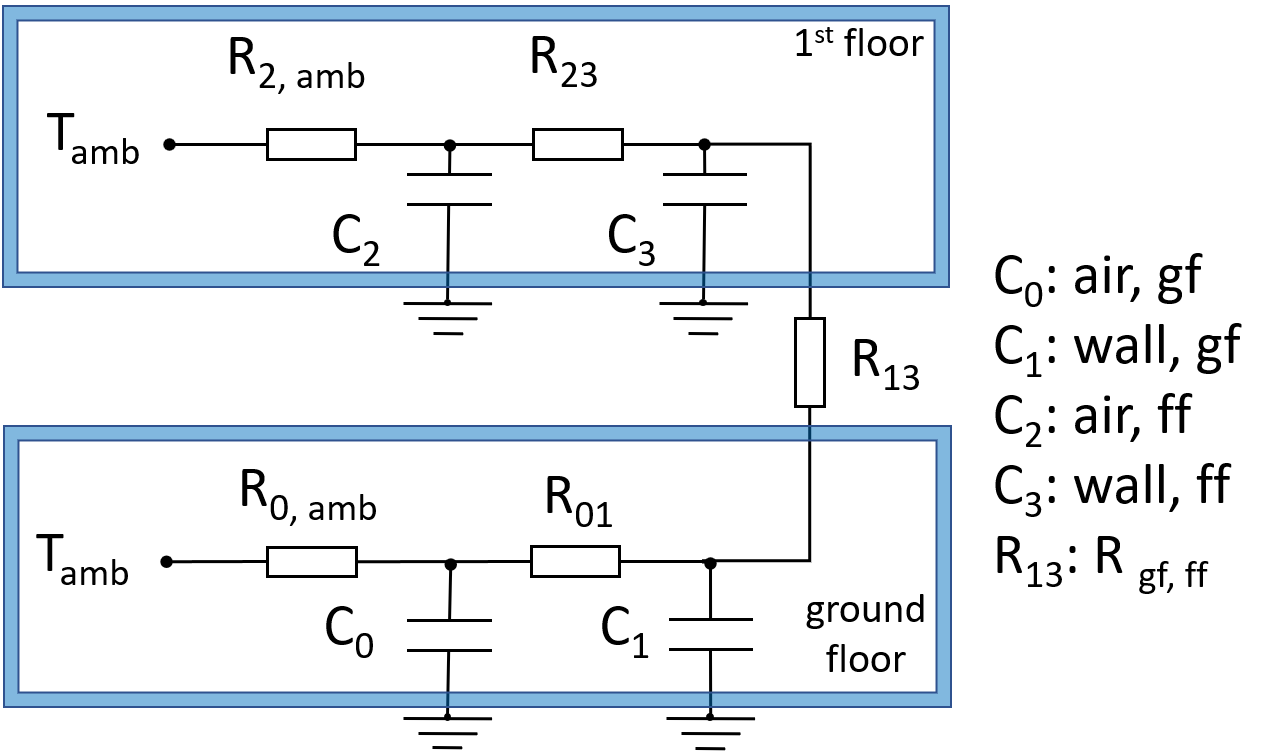
\includegraphics[width=0.6\columnwidth]{Pictures/5R4C_alternative.png}
	\caption[Short title]{5R-4C house model, alternative representation}
	\label{fig:alt5R4C}
\end{figure}

As can be seen in the matrices below, adding $R_{13}$ to the ground floor and first floor "chains" results in a non-symmetric matrix. It has to determined if this disadvantage outweighs the benefit of adding "chains".

\begin{equation}
	\mathbf{C} \cdot \boldsymbol{\dot{\theta}} =
	\begin{bmatrix}
		C_{0} & 0 & 0 & 0\\
		0 &  C_{1} & 0 & 0 \\
		0 & 0 & C_{2} & 0\\
		0 & 0 & 0 & C_{3}
	\end{bmatrix}
	\cdot
	\begin{bmatrix}
		\frac{dT_{0}}{dt} \\
		\frac{dT_{1}}{dt} \\
		\frac{dT_{2}}{dt} \\
		\frac{dT_{3}}{dt} 
	\end{bmatrix}
\end{equation}

\begin{equation}
	\mathbf{K} \cdot \boldsymbol{\theta} =
	\begin{bmatrix}
		\frac{1}{R_{0, amb}} + \frac{1}{R_{01}} & \frac{-1}{R_{01}} & 0 & 0 \\
		\frac{-1}{R_{01}} &  \frac{1}{R_{01}} + \color{red} \frac{1}{R_{13}} & 0 & \color{red} \frac{-1}{R_{13}} \\
		0 & 0 & \frac{1}{R_{2, amb}} + \frac{1}{R_{23}} & \frac{-1}{R_{23}} \\
		0 & \color{red}\frac{-1}{R_{13}} & \frac{-1}{R_{23}}  & \frac{1}{R_{23}} + \color{red}\frac{1}{R_{13}}
	\end{bmatrix}
	\cdot
	\begin{bmatrix}
		T_{0} \\
		T_{1} \\
		T_{2} \\
		T_{3}
	\end{bmatrix}
\end{equation}

\begin{equation}
	\mathbf{\dot{q}} =
	\begin{bmatrix}
		\frac{1}{R_{0, amb}} \cdot T_{amb} + \dot{Q}_{heat, 0} + \dot{Q}_{int, 0} + \dot{Q}_{solar, 0} \\
		\dot{Q}_{solar, 1} \\
		\frac{1}{R_{2, amb}} \cdot T_{amb} + \dot{Q}_{heat, 2} + \dot{Q}_{int, 2} + \dot{Q}_{solar, 2} \\
		\dot{Q}_{solar, 3} 
	\end{bmatrix}
\end{equation}

Renumbering restores the matrices to a symmetric representation:

\begin{figure}[H]
	\centering
	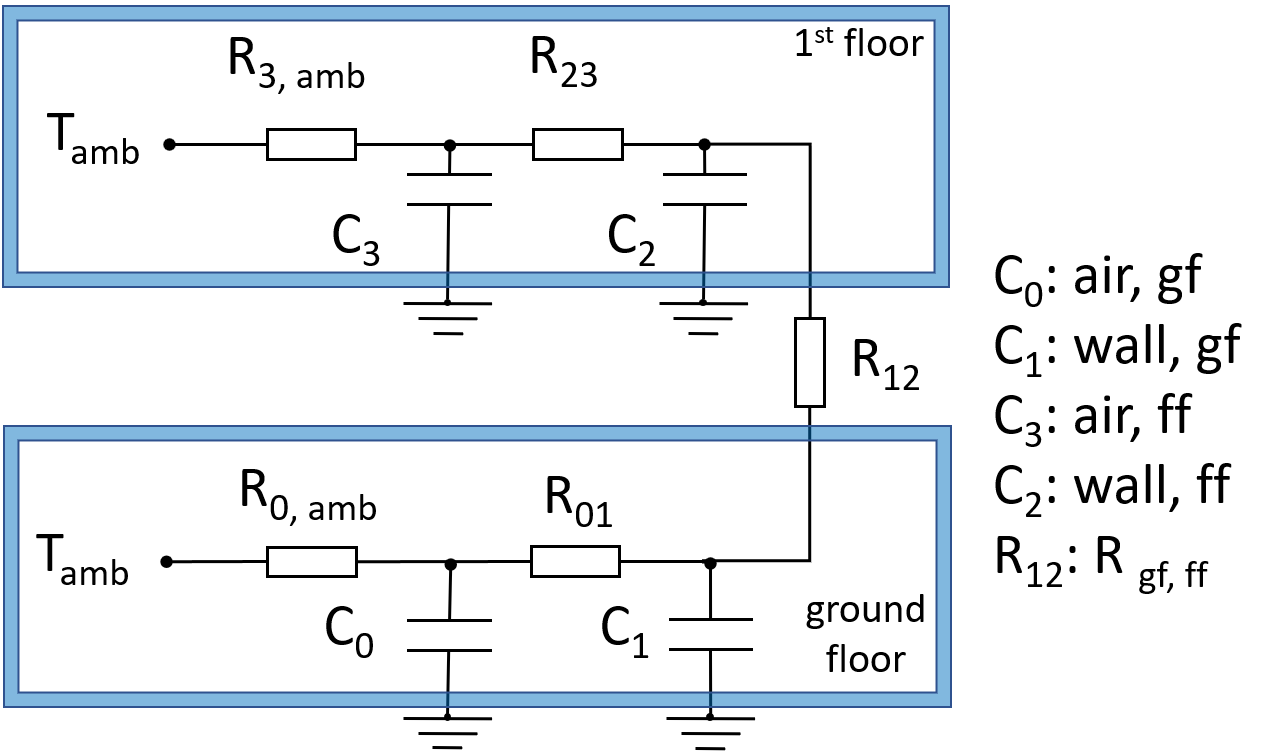
\includegraphics[width=0.6\columnwidth]{Pictures/5R4C_renumbered.png}
	\caption[Short title]{5R-4C house model, alternative representation, renumbered}
	\label{fig:renum5R4C}
\end{figure}

\begin{equation}
	\mathbf{C} \cdot \boldsymbol{\dot{\theta}} =
	\begin{bmatrix}
		C_{0} & 0 & 0 & 0\\
		0 &  C_{1} & 0 & 0 \\
		0 & 0 & C_{2} & 0\\
		0 & 0 & 0 & C_{3}
	\end{bmatrix}
	\cdot
	\begin{bmatrix}
		\frac{dT_{0}}{dt} \\
		\frac{dT_{1}}{dt} \\
		\frac{dT_{2}}{dt} \\
		\frac{dT_{3}}{dt} 
	\end{bmatrix}
\end{equation}

\begin{equation}
	\mathbf{K} \cdot \boldsymbol{\theta} =
	\begin{bmatrix}
		\frac{1}{R_{0, amb}} + \frac{1}{R_{01}} & \frac{-1}{R_{01}} & 0 & 0 \\
		\frac{-1}{R_{01}} &  \frac{1}{R_{01}} + \color{red}\frac{1}{R_{12}} & \color{red}\frac{-1}{R_{12}} & 0 \\
		0 & \color{red} \frac{-1}{R_{12}} & \frac{1}{R_{23}} + \color{red}\frac{1}{R_{12}}   & \frac{-1}{R_{23}}\\
		0 & 0 & \frac{-1}{R_{23}} &  \frac{1}{R_{3, amb}} + \frac{1}{R_{23}} \\
	\end{bmatrix}
	\cdot
	\begin{bmatrix}
		T_{0} \\
		T_{1} \\
		T_{2} \\
		T_{3}
	\end{bmatrix}
\end{equation}

\begin{equation}
	\mathbf{\dot{q}} =
	\begin{bmatrix}
		\frac{1}{R_{0, amb}} \cdot T_{amb} + \dot{Q}_{heat, 0} + \dot{Q}_{int, 0} + \dot{Q}_{solar, 0} \\
		\dot{Q}_{solar, 1} \\
		\dot{Q}_{solar, 2} \\
		\frac{1}{R_{3, amb}} \cdot T_{amb} + \dot{Q}_{heat, 3} + \dot{Q}_{int, 3} + \dot{Q}_{solar, 3}
	\end{bmatrix}
\end{equation}
		
\subsection{2R-2C model with buffervessel}

The "air" and "wall" nodes of the 2R2C model can be extended with "radiator" node. The radiator has a finite heat capacity of itself. Instead of a thermal resistance, the radiator heat exchange in $W/K$ is entered in the model. The radiator emits heat to the "air" node only. In its turn, the radiator is fed from a "buffervessel" node. The buffervessel loses heat to the radiator and is heated up by a gas boiler or alternatively a heat pump. The gas boiler does not heat the house directly, as was the case in the simplest model. A schematic view is given in Fig. \ref{fig:elecbuffer}.

\begin{figure}[H]
	\centering
	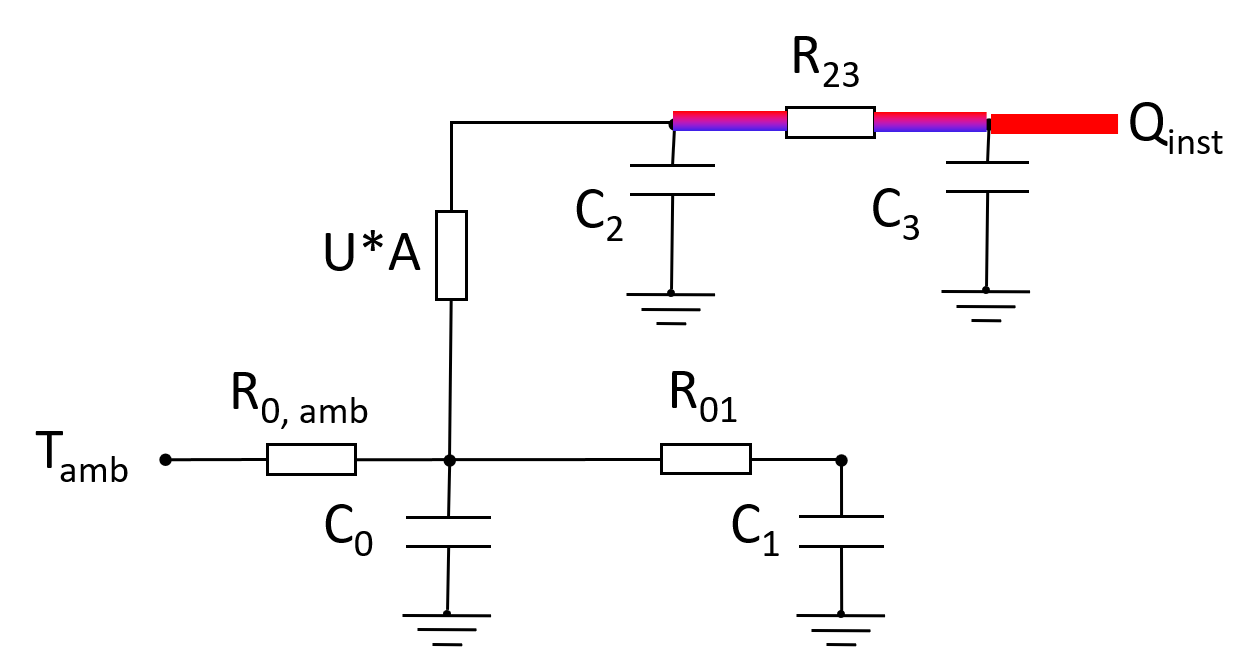
\includegraphics[width=0.7\columnwidth]{Pictures/buffervessel.png}
	\caption[Short title]{2R-2C house model with radiator and buffer vessel}
	\label{fig:buffervessel}
\end{figure} 

The differential equations for heat transport in the model of Fig. \ref{fig:elecbuffer} are:

\begin{equation}
	\begin{aligned}
	    C_{air} \frac{dT_{air}}{dt} &= \frac{T_{outdoor}-T_{air}}{R_{air_{\_}outdoor}} + \frac{T_{wall}-T_{air}}{R_{air_{\_}wall}} + U_{rad} \cdot A_{rad} \cdot (T_{return} - T_{air}) + \dot{Q}_{internal} + \dot{Q}_{solar, 0} \\
	    C_{wall} \frac{dT_{wall}}{dt} &= \frac{T_{air}-T_{wall}}{R_{air_{\_}wall}} + \dot{Q}_{solar, 1} \\
	    C_{rad} \frac{dT_{return}}{dt} &= \dot{m} \cdot c_{p, water} \cdot (T_{buffer} - T_{return}) + U_{rad} \cdot A_{rad} \cdot (T_{air} - T_{return}) \\
		C_{buffer} \frac{dT_{buffer}}{dt} &= \dot{m} \cdot c_{p, water} \cdot ( T_{return} - T_{buffer} ) + \dot{Q}_{inst} \\
	    \frac{dE}{dt} &= \dot{Q}_{inst}
	\end{aligned}
\end{equation}

 A fifth equation, integrating the heat source energy is sometimes added. Re-arranging the terms in the equation gives:
 
\begin{equation}
	\begin{aligned}
		C_{air} \frac{dT_{air}}{dt} &= \left[ \frac{-1}{R_{air_{\_}outdoor}} + \frac{-1}{R_{air_{\_}wall}} +  -1 \cdot U_{rad} \cdot A_{rad} \right] \cdot T_{air} + \frac{T_{wall}}{R_{air_{\_}wall}} + U_{rad} \cdot A_{rad} \cdot T_{return} + \\
		 & \frac{T_{outdoor}}{R_{air_{\_}outdoor}}  + \dot{Q}_{internal} + \dot{Q}_{solar, 0} \\
		C_{wall} \frac{dT_{wall}}{dt} &= \frac{1}{R_{air_{\_}wall}} \cdot T_{air} + \frac{-1}{R_{air_{\_}wall}} \cdot T_{wall} + \dot{Q}_{solar, 1} \\
		C_{rad} \frac{dT_{return}}{dt} &=  U_{rad} \cdot A_{rad} \cdot T_{air} + \left[- U_{rad} \cdot A_{rad} -\dot{m} \cdot c_{p, water}\right] \cdot T_{return} + \dot{m} \cdot c_{p, water} \cdot T_{buffer}\\
		C_{buffer} \frac{dT_{buffer}}{dt} &= \dot{m} \cdot c_{p, water} \cdot T_{return} - \dot{m} \cdot c_{p, water} \cdot T_{buffer} + \dot{Q}_{heat, 3} \\
		\frac{dE}{dt} &= \dot{Q}_{inst}
	\end{aligned}
\end{equation}
Conversion of the equations to a matrix equation yields:
\begin{equation}
	\mathbf{C} \cdot \boldsymbol{\dot{\theta}} =
	\begin{bmatrix}
		C_{0} & 0 & 0 & 0\\
		0 &  C_{1} & 0 & 0 \\
		0 & 0 & C_{2} & 0\\
		0 & 0 & 0 & C_{3}
	\end{bmatrix}
	\cdot
	\begin{bmatrix}
		\frac{dT_{0}}{dt} \\
		\frac{dT_{1}}{dt} \\
		\frac{dT_{2}}{dt} \\
		\frac{dT_{3}}{dt} 
	\end{bmatrix}
\end{equation}

\begin{equation}
	\mathbf{K} \cdot \boldsymbol{\theta} =
	\begin{bmatrix}
		\frac{1}{R_{0, amb}} + \frac{1}{R_{01}} + U \cdot A & \frac{-1}{R_{01}} & -U \cdot A & 0 \\
		\frac{-1}{R_{01}} &  \frac{1}{R_{01}}  & 0 & 0 \\
		-U \cdot A & 0 & U \cdot A + \frac{1}{R_{23}}  & \frac{-1}{R_{23}}\\
		0 & 0 & \frac{-1}{R_{23}} &  \frac{1}{R_{23}} \\
	\end{bmatrix}
	\cdot
	\begin{bmatrix}
		T_{0} \\
		T_{1} \\
		T_{2} \\
		T_{3}
	\end{bmatrix}
\end{equation}

\begin{equation}
	\mathbf{\dot{q}} =
	\begin{bmatrix}
		\frac{1}{R_{0, amb}} \cdot T_{amb} + \dot{Q}_{int, 0} + \dot{Q}_{solar, 0} \\
		\dot{Q}_{solar, 0} \\
		0 \\
		\dot{Q}_{heat, 3}
	\end{bmatrix}
\end{equation}

\subsection{2R-2C model with radiator only}

\begin{figure}[H]
	\centering
	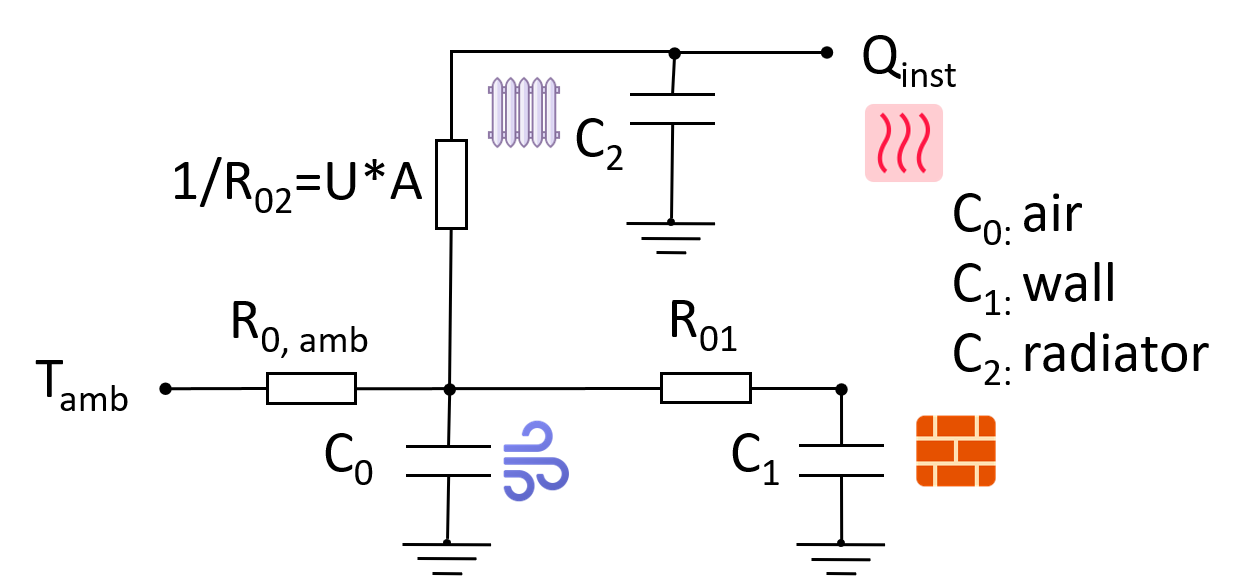
\includegraphics[width=0.7\columnwidth]{Pictures/2R2C_radiator.png}
	\caption[Short title]{2R-2C house model with radiator only}
	\label{fig:2R2Cradiator}
\end{figure} 

The rate of heat transfer from a radiator to the ambient(room) air can be calculated as follows \cite{heatemissionrad}:

\begin{equation}
	\begin{aligned}
	    P & = P_{50} \cdot \left[\Delta T_{LMTD} \cdot \frac{1}{49.32}\right]^n \\
	    \Delta T_{LMTD} & = \frac{ T_{inlet} - T_{return} }{\ln \frac{ T_{inlet} - T_{ambient} }{T_{return} - T_{ambient}}} \\
	    n & = 1.33
    \end{aligned}
\end{equation}

This is sometimes simplified to:

\begin{equation}
	\begin{aligned}
		P & = U \cdot A \cdot \Delta T_{LMTD} \\
		\Delta T_{LMTD} & = \frac{ T_{inlet} - T_{return} }{\ln \frac{ T_{inlet} - T_{ambient} }{T_{return} - T_{ambient}}}
	\end{aligned}
\end{equation}

or simplified to \cite{NEN442, OEM442}:

\begin{equation}
	\begin{aligned}
		P & = K_m \cdot \Delta T^n \\
		\Delta T & = \frac{ T_{inlet} + T_{return} }{2} - {T_{ambient}}
	\end{aligned}
\end{equation}

The differential equations for heat transport in the model of Fig.~\ref{fig:2R2Cradiator} are:

\begin{equation}
	\begin{aligned}
		C_{air} \frac{dT_{air}}{dt} &= \frac{T_{outdoor}-T_{air}}{R_{air_{\_}outdoor}} + \frac{T_{wall}-T_{air}}{R_{air_{\_}wall}} + U_{rad} \cdot A_{rad} \cdot (T_{rad} - T_{air}) + \dot{Q}_{internal} + \dot{Q}_{solar, 0} \\
		C_{wall} \frac{dT_{wall}}{dt} &= \frac{T_{air}-T_{wall}}{R_{air_{\_}wall}} + \dot{Q}_{solar, 1} \\
		C_{rad} \frac{dT_{rad}}{dt} &= \dot{Q}_{inst} + U_{rad} \cdot A_{rad} \cdot (T_{air} - T_{rad}) \\
	\end{aligned}
\end{equation}

Re-arranging the terms in the equation gives:

\begin{equation}
	\begin{aligned}
		C_{air} \frac{dT_{air}}{dt} &= \left[ \frac{-1}{R_{air_{\_}outdoor}} + \frac{-1}{R_{air_{\_}wall}} +  -1 \cdot U_{rad} \cdot A_{rad} \right] \cdot T_{air} + \frac{T_{wall}}{R_{air_{\_}wall}} +  U_{rad} \cdot A_{rad} \cdot T_{rad} + \\
		& \frac{T_{outdoor}}{R_{air_{\_}outdoor}}  + \dot{Q}_{internal} + \dot{Q}_{solar, 0} \\
		C_{wall} \frac{dT_{wall}}{dt} &= \frac{1}{R_{air_{\_}wall}} \cdot T_{air} + \frac{-1}{R_{air_{\_}wall}} \cdot T_{wall} + \dot{Q}_{solar, 1} \\
		C_{rad} \frac{dT_{rad}}{dt} &=  U_{rad} \cdot A_{rad} \cdot T_{air} - U_{rad} \cdot A_{rad} \cdot T_{rad} + \dot{Q}_{heat, 2}\\
	\end{aligned}
\end{equation}
Conversion of the equations to a matrix equation yields:
\begin{equation}
	\mathbf{C} \cdot \boldsymbol{\dot{\theta}} =
	\begin{bmatrix}
		C_{0} & 0 & 0 \\
		0 &  C_{1} & 0  \\
		0 & 0 & C_{2} 
	\end{bmatrix}
	\cdot
	\begin{bmatrix}
		\frac{dT_{0}}{dt} \\
		\frac{dT_{1}}{dt} \\
		\frac{dT_{2}}{dt} 
	\end{bmatrix}
\end{equation}

\begin{equation}
	\mathbf{K} \cdot \boldsymbol{\theta} =
	\begin{bmatrix}
		\frac{1}{R_{0, amb}} + \frac{1}{R_{01}} + U \cdot A & \frac{-1}{R_{01}} & -U \cdot A  \\
		\frac{-1}{R_{01}} &  \frac{1}{R_{01}}  & 0  \\
		-U \cdot A & 0 & U \cdot A 
	\end{bmatrix}
	\cdot
	\begin{bmatrix}
		T_{0} \\
		T_{1} \\
		T_{2}
	\end{bmatrix}
\end{equation}

\begin{equation}
	\mathbf{\dot{q}} =
	\begin{bmatrix}
		\frac{1}{R_{0, amb}} \cdot T_{amb} + \dot{Q}_{int, 0} + \dot{Q}_{solar, 0} \\
		\dot{Q}_{solar, 1} \\
		\dot{Q}_{heat, 2}
	\end{bmatrix}
\end{equation}


\begin{figure}[H]
	\centering
	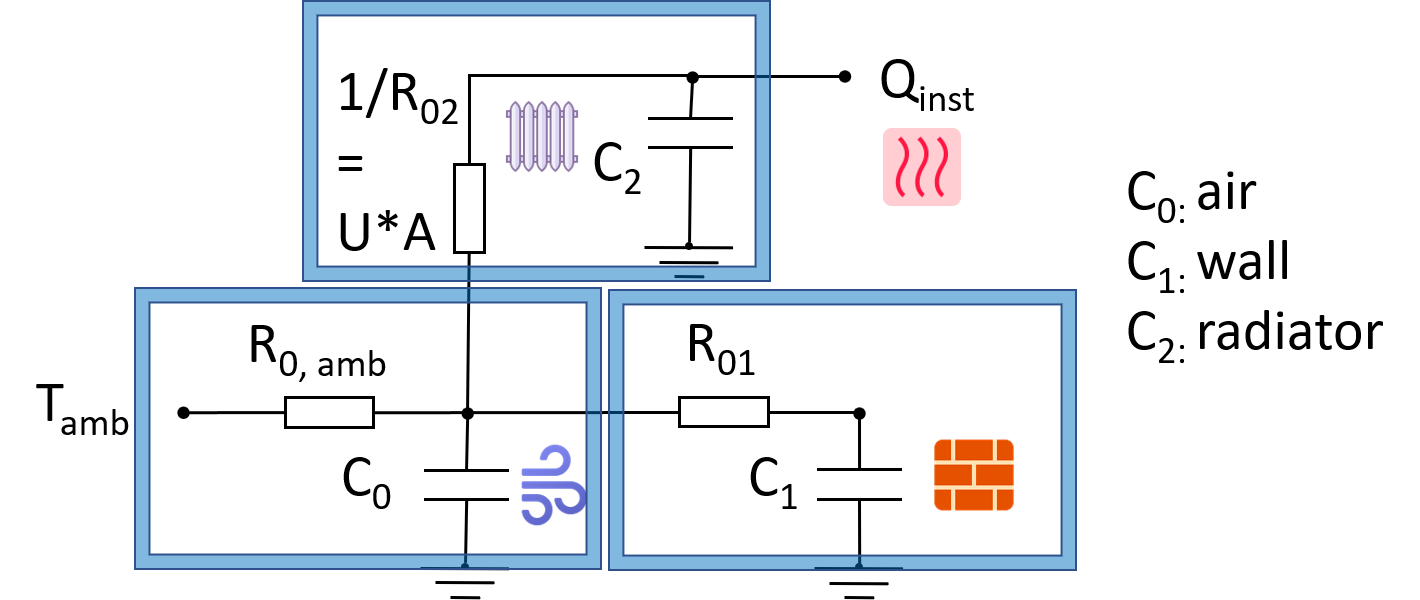
\includegraphics[width=0.7\columnwidth]{Pictures/2R2C_radiator_chains.png}
	\caption[Short title]{2R-2C house model with radiator in 3 chains}
	\label{fig:2R2Cradiator_chains}
\end{figure} 

Starting with the basic 2R2C model we write down the matrices. Note that the heat source for the house is omitted at first. Solar energy entering the house is partitioned between air and wall, Heat generated due to the presence and activities of inhabitants is added to the air node:

\begin{equation}
	\mathbf{C} \cdot \boldsymbol{\dot{\theta}} =
	\begin{bmatrix}
		C_{0} & 0 \\
		0 &  C_{1}
	\end{bmatrix}
	\cdot
	\begin{bmatrix}
		\frac{dT_{0}}{dt} \\
		\frac{dT_{1}}{dt}
	\end{bmatrix}
\end{equation}

\begin{equation}
	\mathbf{K} \cdot \boldsymbol{\theta} =
	\begin{bmatrix}
		\frac{1}{R_{0, amb}} + \frac{1}{R_{01}} & \frac{-1}{R_{01}} \\
		\frac{-1}{R_{01}} &  \frac{1}{R_{01}}
	\end{bmatrix}
	\cdot
	\begin{bmatrix}
		T_{0} \\
		T_{1}
	\end{bmatrix}
\end{equation}

\begin{equation}
	\mathbf{\dot{q}} =
	\begin{bmatrix}
		\frac{1}{R_{0, amb}} \cdot T_{amb} + \dot{Q}_{int, 0} + \dot{Q}_{solar, 0} \\
		\dot{Q}_{solar, 1}
	\end{bmatrix}
\end{equation}

As a third link in the chain, a radiator is added, with a heat capacity $C_{rad}$ and a heat delivery $U \cdot A \cdot (T_{rad} - T_{air})$ to the air node. The heat source $\dot{Q}_{inst}$ is now connected to the radiator.

\begin{equation}
	\mathbf{C} \cdot \boldsymbol{\dot{\theta}} =
	\begin{bmatrix}
		C_{0} & 0 & \color{red} 0 \\
		0 &  C_{1} & \color{red} 0  \\
		\color{red} 0 & \color{red} 0 & \color{red} C_{2} 
	\end{bmatrix}
	\cdot
	\begin{bmatrix}
		\frac{dT_{0}}{dt} \\
		\frac{dT_{1}}{dt} \\
		\color{red}\frac{dT_{2}}{dt} 
	\end{bmatrix}
\end{equation}

\begin{equation}
	\mathbf{K} \cdot \boldsymbol{\theta} =
	\begin{bmatrix}
		\frac{1}{R_{0, amb}} + \frac{1}{R_{01}} {\color{red}+ U \cdot A} & \frac{-1}{R_{01}} & {\color{red}-U \cdot A}  \\
		\frac{-1}{R_{01}} &  \frac{1}{R_{01}}  & \color{red} 0  \\
		{\color{red}-U \cdot A} & \color{red} 0 & {\color{red}U \cdot A }
	\end{bmatrix}
	\cdot
	\begin{bmatrix}
		T_{0} \\
		T_{1} \\
	   \color{red}T_{2}
	\end{bmatrix}
\end{equation}

\begin{equation}
	\mathbf{\dot{q}} =
	\begin{bmatrix}
		\frac{1}{R_{0, amb}} \cdot T_{amb} + \dot{Q}_{int, 0} + \dot{Q}_{solar, 0} \\
		\dot{Q}_{solar, 1} \\
		\color{red} \dot{Q}_{heat, 2}
	\end{bmatrix}
\end{equation}

In this example, it becomes visible (in red) that the rank of the $C$- and $K$-matrix, and the $\dot{q}$-vector is extended by 1. The heat capacity of the radiator is included as an extra \emph{diagonal} element in the $C$-matrix. The heat delivery from the radiator to the indoor air is added to or subtracted from the {00}, {22}, {02} and {20} elements of th $K$-matrix, so that it remains a \emph{symmetric} matrix. The heater is connected to the radiator, represented by element {2} of the $\dot{q}$-vector. 
%\usepackage{xcolor}

\subsection{2R2C revisited: 2R3C}
\label{sec:2R3C}
The 2R2C model as represented in \ref{fig:elec2R2C} treats the node of the outside temperature ($T_{amb}$) differently from the other nodes, $T_{air}$ and $T_{walls}$.  This representation is inconsistent, and actually incomplete. Implicitly, the model links a source/sink to the node that controls the outdoor temperature. In literature, one can find models in which this source has been made explicit, such as in \cite{achterbos}. It seems that this representation has been lost over time. 

In order to complete the analogy with the other nodes in the model we can connect an additional capacitor ($C_{amb}$). The capacity will be tending to infinity, as we assume the outside temperature does not  change due to heat exchange with the house.

\todo{todo:figure including a source and capacitor}

Adding the capacitor and the source also will change the equations. Actually, it results in a more structured set of equations. The equations will be as follows:
\begin{equation}
	\mathbf{C} \cdot \boldsymbol{\dot{\theta}} =
	\begin{bmatrix}
		C_{amb} & 0 & 0\\
		0 &  C_{air} & 0   \\
		0 & 0 & C_{wall} 
	\end{bmatrix}
	\cdot
	\begin{bmatrix}
		\frac{dT_{amb}}{dt} \\
		\frac{dT_{air}}{dt} \\
		\frac{dT_{wall}}{dt} 
	\end{bmatrix}
\end{equation}

\begin{equation}
	\mathbf{K} \cdot \boldsymbol{\theta} =
	\begin{bmatrix}
		\frac{1}{R_{amb, air}}  & \frac{-1}{R_{amb,air}} & 0  \\
		\frac{-1}{R_{amb, air}} &  \frac{1}{R_{amb, air}} + \frac{1}{R_{air,wall}} &  \frac{-1}{R_{air,wall}} \\
		 0 & \frac{-1}{R_{air, wall}}  & \frac{1}{R_{air,wall}} 
	\end{bmatrix}
	\cdot
	\begin{bmatrix}
		T_{amb} \\
		T_{air} \\
		T_{wall}
	\end{bmatrix}
\end{equation}

\begin{equation}
	\mathbf{\dot{q}} =
	\begin{bmatrix}
		\dot{Q}_{amb}\\
		\dot{Q}_{air} \\
		\dot{Q}_{wall} 
	\end{bmatrix}
\end{equation}

In the equations we now see that the matrix $K$ represents the interaction between the different heat capacities.  The off-diagonal elements are equal to (minus) conductance factor $\frac{-1}{R}$ between the respective connected nodes. The structure of $K$ is such that the sum over the rows will always be zero, where the diagonal elements equal the negative sum of the off-diagonal elements.

The vector $\dot{q}$ contains all heat sources (and sinks). 

Generalizing the idea above, alternative models can be easily constructed using an underlying graph. In the graph each node is labeled with a heat capacity $C_i$, and temperature $T_i$. Nodes $i$ and $j$ can be connected by an edge labeled with $R_{i,j}$, where $\frac{1}{R_{i,j}}$ represents the heat conductance between the two nodes. The $K$-matrix is the connectivity matrix of the graph, where $K_{i,j} = \frac{-1}{R_{i,j}}$. The diagonal elements, $K{i,i}$ are set such that the sums over the rows will be equal to zero.
 

Additionally, each node can be connected to a source (or sink). Two types of sources are available. A "temperature source" represents a source that will keep the temperature of the connected node constant. This source type can be used to set the ambient temperature.   

A heat source represents a source that will provide a continuous constant energy flow into the node. This source type can be used to represent the inflow of energy by for example the sun. 

\subsubsection{example: 2R-2C house with buffer}

   
\subsection{3R2C model}

For an apartment building, the simplest model has two nodes with a finite heat capacity, the interior and the building construction. Both nodes have a finite thermal resistance to the ambient environment. Finally there is a thermal resistance between the nodes. Graphically, the model is represented by Figure~\ref{fig:3R2C}

\begin{figure}[H]
	\centering
	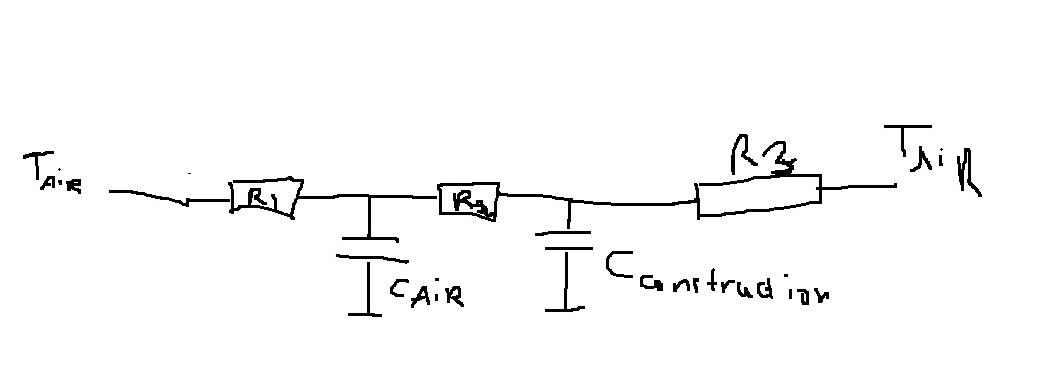
\includegraphics[width=0.7\columnwidth]{Pictures/3R2Cmodel}
	\caption[Short title]{3R-2C house model}
	\label{fig:3R2C}
\end{figure} 

The differential equations are:

\begin{equation}
	\begin{aligned}
		C_{air}\frac{dT_{air}}{dt} &=\frac{T_{amb}-T_{air}}{R_{air, amb}} + \frac{T_{wall}-T_{air}}{R_{air, wall}} + \dot{Q}_{heat, air} + \dot{Q}_{int, air} + \dot{Q}_{solar, air} 
		\\ \\
		C_{wall}\frac{dT_{wall}}{dt} &=\frac{T_{air}-T_{wall}}{R_{air, wall}} + \frac{T_{amb}-T_{wall}}{R_{wall, amb}} +\dot{Q}_{solar, wall}
	\end{aligned}
\end{equation}

Writing out the differential equations in the classical notation:

\begin{equation}
	\begin{aligned}
		C_{air}\frac{dT_{air}}{dt} &= \left[ \frac{-1}{R_{air, amb}} + \frac{-1}{R_{air, wall}} \right]  \cdot T_{air}  + \frac{1}{R_{air, wall}} \cdot T_{wall} + \frac{1}{R_{air, amb}} \cdot T_{amb} + \dot{Q}_{heat, air} + \dot{Q}_{int, air} + \dot{Q}_{solar, air} 
		\\ \\
		C_{wall}\frac{dT_{wall}}{dt} &= \frac{1}{R_{air, wall}} \cdot T_{air} + \left[ \frac{-1}{R_{wall, amb}} + \frac{-1}{R_{air, wall}} \right]  \cdot T_{wall} + \frac{1}{R_{wall, amb}} \cdot T_{amb} + \dot{Q}_{solar, wall}
	\end{aligned}
\end{equation}

The differential equations can be written in matrix notation as:

\begin{subequations}
	\label{eq:matnot}
	\begin{align}
		\mathbf{C} \cdot \boldsymbol{\dot{\theta}} = - \mathbf{K} \cdot \boldsymbol{\theta} + \mathbf{\dot{q}} \\ 
		\mathbf{C} \cdot \boldsymbol{\dot{\theta}} + \mathbf{K} \cdot \boldsymbol{\theta} = \mathbf{\dot{q}}
	\end{align}
\end{subequations}

with:

\begin{equation}
	\mathbf{C} \cdot \boldsymbol{\dot{\theta}} =
	\begin{bmatrix}
		C_{air} & 0 \\
		0 &  C_{wall}
	\end{bmatrix}
	\cdot
	\begin{bmatrix}
		\frac{dT_{air}}{dt} \\
		\frac{dT_{wall}}{dt}
	\end{bmatrix}
\end{equation}

\begin{equation}
	\mathbf{K} \cdot \boldsymbol{\theta} =
	\begin{bmatrix}
		\frac{1}{R_{air, amb}} + \frac{1}{R_{air, wall}} & \frac{-1}{R_{air, wall}} \\
		\frac{-1}{R_{air, wall}} &  \frac{1}{R_{wall, amb}} + \frac{1}{R_{air, wall}}
	\end{bmatrix}
	\cdot
	\begin{bmatrix}
		T_{air} \\
		T_{wall}
	\end{bmatrix}
\end{equation}

\begin{equation}
	\mathbf{\dot{q}} =
	\begin{bmatrix}
		\frac{1}{R_{air, amb}} \cdot T_{amb} + \dot{Q}_{heat, air} + \dot{Q}_{int, air} + \dot{Q}_{solar, air} \\
		\frac{1}{R_{wall, amb}} \cdot T_{amb} + \dot{Q}_{solar, wall}
	\end{bmatrix}
\end{equation}

Written out, the differential equation according to \eqref{eq:matnot} becomes:

\begin{equation}
	\begin{aligned}
		\begin{bmatrix}
			C_{air} & 0 \\
			0 &  C_{wall}
		\end{bmatrix}
		\cdot
		\begin{bmatrix}
			\frac{dT_{air}}{dt} \\
			\frac{dT_{wall}}{dt}
		\end{bmatrix}
		=
		\begin{bmatrix}
			\frac{-1}{R_{air, amb}} + \frac{-1}{R_{air, wall}} & \frac{1}{R_{air, wall}} \\
			\frac{1}{R_{air, wall}} &  \frac{-1}{R_{wall, amb}} + \frac{-1}{R_{air, wall}}
		\end{bmatrix}
		\cdot
		\begin{bmatrix}
			T_{air} \\
			T_{wall}
		\end{bmatrix}
		+ \\ \\
		\begin{bmatrix}
			\frac{1}{R_{air, amb}} \cdot T_{amb} + \dot{Q}_{heat, air} + \dot{Q}_{int, air} + \dot{Q}_{solar, air} \\
			\frac{1}{R_{air, amb}} \cdot T_{amb} + \dot{Q}_{solar, wall}
		\end{bmatrix}
	\end{aligned}
\end{equation}

In the alternative notation:

\begin{equation}
	\begin{aligned}
		\begin{bmatrix}
			C_{air} & 0 \\
			0 &  C_{wall}
		\end{bmatrix}
		\cdot
		\begin{bmatrix}
			\frac{dT_{air}}{dt} \\
			\frac{dT_{wall}}{dt}
		\end{bmatrix}
		+
		\begin{bmatrix}
			\frac{1}{R_{air, amb}} + \frac{1}{R_{air, wall}} & \frac{-1}{R_{air, wall}} \\
			\frac{-1}{R_{air, wall}} &  \frac{1}{R_{wall, amb}} + \frac{1}{R_{air, wall}}
		\end{bmatrix}
		\cdot
		\begin{bmatrix}
			T_{air} \\
			T_{wall}
		\end{bmatrix}
		= \\ \\
		\begin{bmatrix}
			\frac{1}{R_{air, amb}} \cdot T_{amb} + \dot{Q}_{heat, air} + \dot{Q}_{int, air} + \dot{Q}_{solar, air} \\
			\frac{1}{R_{wall, amb}} \cdot T_{amb} + \dot{Q}_{solar, wall}
		\end{bmatrix}
	\end{aligned}
\end{equation}

it is clear that in this example, where multiple nodes in the thermal network are connected to the ambient surroundings, the approach of Section~\ref{sec:2R3C} becomes more adventageous:

\subsection{3R3C model}

The previous 3R2C model representation necessitates an \emph{ad hoc} term in the heat supply vector $\mathbf{\dot{q}}$. Analogous to Section~\ref{sec:2R3C}, we can include the ambient surroundings as a (large) heat capacity into the model. This will change the 3R2C model into a 3R3C model. The equations become:

\begin{equation}
	\mathbf{C} \cdot \boldsymbol{\dot{\theta}} =
	\begin{bmatrix}
		C_{amb} & 0 & 0\\
		0 &  C_{air} & 0   \\
		0 & 0 & C_{wall} 
	\end{bmatrix}
	\cdot
	\begin{bmatrix}
		\frac{dT_{amb}}{dt} \\
		\frac{dT_{air}}{dt} \\
		\frac{dT_{wall}}{dt} 
	\end{bmatrix}
\end{equation}

For $\mathbf{K}$ we can start with filling out the non-diagonal symmetic matrix elements:

\begin{equation}
		\mathbf{K} =
	\begin{bmatrix}
		0  & \frac{-1}{R_{amb,air}} & \frac{-1}{R_{amb,wall}}  \\
		\frac{-1}{R_{amb, air}} &  0 &  \frac{-1}{R_{air,wall}} \\
		\frac{-1}{R_{amb,wall}} & \frac{-1}{R_{air, wall}}  & 0 
	\end{bmatrix}
\end{equation}

Then we can complete the diagonal elements, so that the sum over each row becomes zero:

\begin{equation}
	\mathbf{K} \cdot \boldsymbol{\theta} =
	\begin{bmatrix}
		\frac{1}{R_{amb, air}} + \frac{1}{R_{air,wall}}  & \frac{-1}{R_{amb,air}} & \frac{-1}{R_{amb,wall}}  \\
		\frac{-1}{R_{amb, air}} &  \frac{1}{R_{amb, air}} + \frac{1}{R_{air,wall}} &  \frac{-1}{R_{air,wall}} \\
		\frac{-1}{R_{amb,wall}} & \frac{-1}{R_{air, wall}}  & \frac{1}{R_{amb, wall}} + \frac{1}{R_{air,wall}} 
	\end{bmatrix}
	\cdot
	\begin{bmatrix}
		T_{amb} \\
		T_{air} \\
		T_{wall}
	\end{bmatrix}
\end{equation}

\begin{equation}
	\mathbf{\dot{q}} =
	\begin{bmatrix}
		\dot{Q}_{amb}\\
		\dot{Q}_{air} \\
		\dot{Q}_{wall} 
	\end{bmatrix}
\end{equation}

\subsection{Coupling the housemodel elements}

The housemodel is to be extended with modular elements representing the installations that supply the heat demanded by the building. Each subsystem contributes its own set of differential equations to the total system. In Fig.~\ref{fig:grandmodel}, the subsystems are indicated with a color code.
 
\begin{figure}[H]
	\centering
	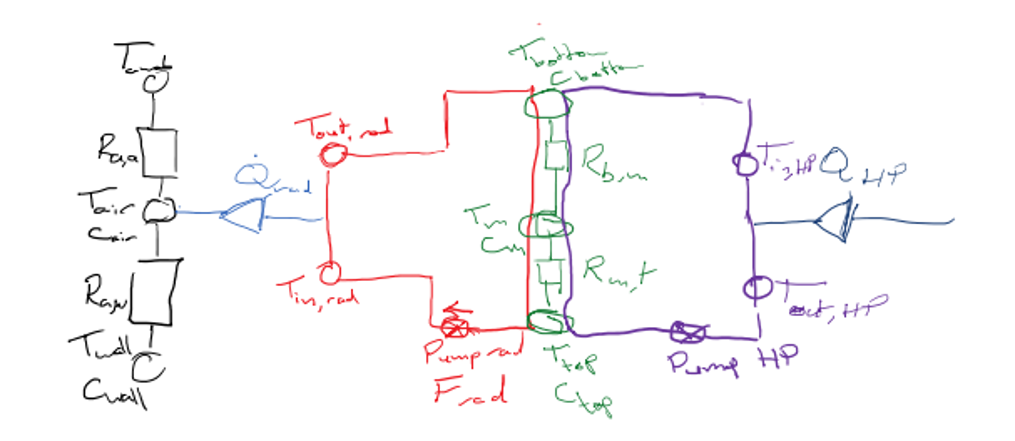
\includegraphics[width=0.9\columnwidth]{Pictures/grand_model}
	\caption[Short title]{Grand Model}
	\label{fig:grandmodel}
\end{figure} 

The building itself, in black, generates the differential equations:

\begin{equation}
	\begin{aligned}
		T_{air} \text{:} \quad C_{air}\frac{dT_{air}}{dt} &=\frac{T_{amb}-T_{air}}{R_{air, amb}} + \frac{T_{wall}-T_{air}}{R_{air, wall}} + \dot{Q}_{rad, air} 
		\\ \\
		T_{wall} \text{:} \quad C_{wall}\frac{dT_{wall}}{dt} &=\frac{T_{air}-T_{wall}}{R_{air, wall}}
	\end{aligned}
\end{equation}

$T_{amb}$: given as piecewise constant function, in interval $[t_i, t_{i+1}]$, $T_{amb} = T_{amb, i}$

The radiator element, coupled to the node $T_{air}$, transfers heat to the building at a rate $\dot{Q}_{rad}$. It has a feed temperature $T_{feed}$ and a return temperature $T_{return}$. The radiator is modeled as a "cross-flow" heat exchanger, obeying the "radiator equation":

{\color{blue}
\begin{equation}
	\begin{aligned}
		\dot{Q}_{rad} \text{:} \quad \dot{Q}_{rad} &= C_{rad} \cdot (\Delta T_{LMTD})^n \text{, with } \Delta T_{LMTD} = \frac{T_{feed} - T_{return}}{\ln\left(\frac{T_{feed} -T_{air}}{T_{return} - T_{air}}\right)}
		\\ \\
	    \text{also, :} \quad \dot{Q}_{rad} &= F_{rad} \cdot c_w \cdot (T_{feed} - T_{return})
	\end{aligned}
\end{equation}
}

when $T_{feed}$, $T_{air}$ and $F_{rad}$ are known, we have two equations with two unknowns $\dot{Q}_{rad}$ and $T_{return}$.

{\color{red}Question: when do you solve this system? Do you need to solve this within the time interval $[t_i, t_{i+1}]$?}

Further equations:

\begin{equation}
	\begin{aligned}
        {\color{red}T_{feed}} &= {\color{teal}T_{top}} \\
        {\color{red}T_{return}} & \text{ should follow from equations above.}
    \end{aligned}
\end{equation}

{\color{teal}
\begin{equation}
	\label{eq:buffer}
	\begin{aligned}
	T_{top} \text{:} \quad C_{top}\frac{dT_{top}}{dt} &= \frac{T_{top}-T_{mid}}{-R_{mid, top}} + F_{HP} \cdot c_w \cdot (T_{HP,out} - T_{top}) + \max(F_{rad}-F_{HP}, 0) \cdot c_w \cdot (T_{mid} - T_{top})
    \\ \\
    T_{mid} \text{:} \quad C_{mid}\frac{dT_{mid}}{dt} &= \frac{T_{top}-T_{mid}}{R_{mid, top}} + \frac{T_{mid}-T_{bot}}{-R_{bot, mid}} + \\
    & \max(F_{HP}-F_{rad}, 0) \cdot c_w \cdot (T_{top} - T_{mid}) + \max(F_{rad}-F_{HP}, 0) \cdot c_w \cdot (T_{mid} - T_{bot}) 
    \\ \\
    T_{bot} \text{:} \quad C_{bot}\frac{dT_{bot}}{dt} &= \frac{T_{mid}-T_{bot}}{R_{bot, mid}} + F_{rad} \cdot c_w \cdot (T_{return} - T_{bot}) + \\
    & \max(F_{HP}-F_{rad}, 0) \cdot c_w \cdot (T_{mid} - T_{bot})
	\end{aligned}
\end{equation}
}

\begin{equation}
	\begin{aligned}
		T_{HP,in} &= {\color{teal}T_{bot}} \\
		T_{HP,out} \text{:} \quad \dot{Q}_{HP} &= F_{HP} \cdot c_w \cdot (T_{HP,out} - T_{HP,in}
		\dot{Q}_{HP} &= f(T_{HP,in}\text{,} T_{HP,out}\text{,} T_{src,in}\text{,} T_{src,out}))
	\end{aligned}
\end{equation}

{\color{red} heat pump function? Also here the question is: when to solve this equation?}


Writing out the differential equations in the classical notation:

\begin{equation}
	\begin{aligned}
		C_{air}\frac{dT_{air}}{dt} &= \left[ \frac{-1}{R_{air, amb}} + \frac{-1}{R_{air, wall}} \right]  \cdot T_{air}  + \frac{1}{R_{air, wall}} \cdot T_{wall} + \frac{1}{R_{air, amb}} \cdot T_{amb} + \dot{Q}_{heat, air}
		\\ \\
		C_{wall}\frac{dT_{wall}}{dt} &= \frac{1}{R_{air, wall}} \cdot T_{air} + \frac{-1}{R_{air, wall}}   \cdot T_{wall}
	\end{aligned}
\end{equation}

The differential equations of the 2R-2C house model (in black) be written in matrix notation as:

\begin{subequations}
	\label{eq:matnot}
	\begin{align}
		\mathbf{C} \cdot \boldsymbol{\dot{\theta}} = - \mathbf{K} \cdot \boldsymbol{\theta} + \mathbf{\dot{q}} \\ 
		\mathbf{C} \cdot \boldsymbol{\dot{\theta}} + \mathbf{K} \cdot \boldsymbol{\theta} = \mathbf{\dot{q}}
	\end{align}
\end{subequations}

with:

\begin{equation}
	\mathbf{C} \cdot \boldsymbol{\dot{\theta}} =
	\begin{bmatrix}
		C_{air} & 0 \\
		0 &  C_{wall}
	\end{bmatrix}
	\cdot
	\begin{bmatrix}
		\frac{dT_{air}}{dt} \\
		\frac{dT_{wall}}{dt}
	\end{bmatrix}
\end{equation}

\begin{equation}
	\mathbf{K} \cdot \boldsymbol{\theta} =
	\begin{bmatrix}
		\frac{1}{R_{air, amb}} + \frac{1}{R_{air, wall}} & \frac{-1}{R_{air, wall}} \\
		\frac{-1}{R_{air, wall}} &  \frac{1}{R_{air, wall}}
	\end{bmatrix}
	\cdot
	\begin{bmatrix}
		T_{air} \\
		T_{wall}
	\end{bmatrix}
\end{equation}

\begin{equation}
	\mathbf{\dot{q}} =
	\begin{bmatrix}
		\frac{1}{R_{air, amb}} \cdot T_{amb} + \dot{Q}_{heat, air} \\
		0
	\end{bmatrix}
\end{equation}



The routines in Matlab, Simulink and Python need a \emph{model function} that provides the vector $\boldsymbol{\dot{\theta}}$ for evaluation at any time instance chosen by the algorithm. The equations \eqref{eq:matnot} then should be cast in the following form by left multiplication with $\mathbf{C^{-1}}$.

\begin{subequations}
	\label{eq:matnot_ivp}
	\begin{align}
		\mathbf{C}^{-1} \cdot \mathbf{C} \cdot \boldsymbol{\dot{\theta}} = - \mathbf{C}^{-1} \cdot \mathbf{K} \cdot \boldsymbol{\theta} + \mathbf{C}^{-1} \cdot \mathbf{\dot{q}} \\ 
		\boldsymbol{\dot{\theta}} = - \mathbf{C}^{-1} \cdot \mathbf{K} \cdot \boldsymbol{\theta} + \mathbf{C}^{-1} \cdot \mathbf{\dot{q}}
	\end{align}
\end{subequations}

Since $\mathbf{C}$ is a \emph{diagonal} matrix with positive elements only, its inverse exists and contains the reciprocal elements on its diagonal:

\begin{equation}
	\mathbf{C^{-1}} =
	\begin{bmatrix}
		\frac{1}{C_{air}} & 0 \\
		0 &  \frac{1}{C_{wall}}
	\end{bmatrix}
\end{equation}

This provides the division by the lumped thermal capacitances of the air and wall compartments in the model, necessary for the calculating the derivative vector $\boldsymbol{\dot{\theta}}$ in the model functions. 

Radiator

\begin{equation}
	\begin{aligned}
		C_{feed}\frac{dT_{feed}}{dt} &= F_{rad} \cdot c_w \cdot (T_{top}- T_{feed})
		\\ \\
		C_{return}\frac{dT_{feed}}{dt} &= 
	\end{aligned}
\end{equation} 


\begin{equation}
	\mathbf{C} \cdot \boldsymbol{\dot{\theta}} =
	\begin{bmatrix}
		C_{feed} & 0 \\
		0 &  C_{return}
	\end{bmatrix}
	\cdot
	\begin{bmatrix}
		\frac{dT_{feed}}{dt} \\
		\frac{dT_{return}}{dt}
	\end{bmatrix}
\end{equation}

\begin{equation}
	\mathbf{K} \cdot \boldsymbol{\theta} =
	\begin{bmatrix}
		0 & 0 \\
		0 &  0
	\end{bmatrix}
	\cdot
	\begin{bmatrix}
		T_{feed} \\
		T_{return}
	\end{bmatrix}
\end{equation}

\begin{equation}
	\mathbf{\dot{q}} =
	\begin{bmatrix}
		0 \\
		\dot{Q}_{rad, air}
	\end{bmatrix}
\end{equation}

\subsubsection{Buffer vessel}

The buffer vessel model is the general model for a "stratified (layered) tank". In order to avoid extensive convection in the tank, the model assumes that addition of hot water from the heat source \emph{and} extraction of hot water to the sink (demand) occurs in the \emph{top} layer.  Return flow from the sink is to the \emph{bottom} layer of the vessel.

The differential equations [\ref{eq:buffer}] can be rewritten as:

{\color{teal}
	\begin{equation}
		\begin{aligned}
			C_{top}\frac{dT_{top}}{dt} &= \frac{-1}{R_{mid, top}} (T_{top}-T_{mid}) + \max(F_{rad}-F_{HP}, 0) \cdot (T_{mid} - T_{top}) \\
			&+ F_{HP} \cdot (T_{HP,out} - T_{top})
			\\ \\
			C_{mid}\frac{dT_{mid}}{dt} &= \frac{1}{R_{mid, top}} (T_{top}-T_{mid}) + \frac{-1}{R_{bot, mid}}(T_{mid}-T_{bot}) \\
			& + \max(F_{HP}-F_{rad}, 0) \cdot (T_{top} - T_{mid}) + \max(F_{rad}-F_{HP}, 0)  \cdot (T_{mid} - T_{bot}) 
			\\ \\
			C_{bot}\frac{dT_{bot}}{dt} &= \frac{1}{R_{bot, mid}} (T_{mid}-T_{bot}) + \max(F_{HP} - F_{rad}, 0) \cdot (T_{mid} - T_{bot})\\
			& + F_{rad} \cdot (T_{return} - T_{bot}) 
		\end{aligned}
	\end{equation}
}

These differential equations can be written in matrix notation as previously, but a \emph{convection} matrix $\mathbf{F}$ is added:

\begin{subequations}
	\label{eq:matnot}
	\begin{align}
		\mathbf{C} \cdot \boldsymbol{\dot{\theta}} + \mathbf{K} \cdot \boldsymbol{\theta} + \mathbf{F} \cdot \boldsymbol{\theta}= \mathbf{\dot{q}}
	\end{align}
\end{subequations}

with:

\begin{equation}
	\mathbf{C} \cdot \boldsymbol{\dot{\theta}} =
	\begin{bmatrix}
		C_{top} & 0 & 0 \\
		0 &  C_{mid} & 0 \\
		0 & 0 & C_{bot} \\
	\end{bmatrix}
	\cdot
	\begin{bmatrix}
		\frac{dT_{top}}{dt} \\
		\frac{dT_{mid}}{dt} \\
		\frac{dT_{bot}}{dt}
	\end{bmatrix}
\end{equation}

\begin{equation}
	\mathbf{K} \cdot \boldsymbol{\theta} =
	\begin{bmatrix}
		\frac{1}{R_{mid,top}} & \frac{-1}{R_{mid,top}} & 0\\
		\frac{-1}{R_{mid,top}} &  \frac{1}{R_{mid, top}} + \frac{1}{R_{bot,mid}} & \frac{-1}{R_{bot,mid}}\\
		0 &  \frac{-1}{R_{bot, mid}} & \frac{1}{R_{bot,mid}}
	\end{bmatrix}
	\cdot
	\begin{bmatrix}
		T_{top} \\
		T_{mid} \\
		T_{bot}
	\end{bmatrix}
\end{equation}

\begin{equation}
	\mathbf{F} \cdot \boldsymbol{\theta} =
	\begin{bmatrix}
		F_{HP,out} + F_{rad} & F_{rad} & 0 \\
		F_{rad} &  0  & F_{rad} \\
		0 &  F_{rad} & F_{HP} + F_{rad}
	\end{bmatrix}
	\cdot
	\begin{bmatrix}
		T_{top} \\
		T_{mid} \\
		T_{bot}
	\end{bmatrix}
\end{equation}

\begin{equation}
	\mathbf{\dot{q}} =
	\begin{bmatrix}
		\frac{1}{R_{air, amb}} \cdot T_{amb} + \dot{Q}_{heat, air} \\
		0
	\end{bmatrix}
\end{equation}


F1: [0 1 2 0]

F2: [2 1 0 2]

\begin{equation}
	\mathbf{DF_{F1}} = 
	\begin{bmatrix}
		0 & 1 &-1  \\
	   -1 & 0 & 1  \\
		1 &-1 & 0  \\
	\end{bmatrix}
	\label{eq:DFflow1}
\end{equation}

\begin{equation}
	\mathbf{DF_{F2}} = 
	\begin{bmatrix}
		0 &-1 & 1  \\
	    1 & 0 &-1  \\
	   -1 & 1 & 0  \\
	\end{bmatrix}
	\label{eq:DFflow1}
\end{equation}

In each time step, when the flow sizes have been determined by the control algorithms, each directed-flow-matrix is multiplied by its respected flow size in [$\frac{\text{m}^3}{\text{s}}$]. All resulting matrices can then be added together. Assuming a flow of size $f_1$ and $f_2$ for the flows $F1$ and $F2$, respectively we now get the matrix $\mathbf{SF}$:
\begin{equation}
	\mathbf{SF} = f_1 \cdot \mathbf{DF_{F1}} + f_2 \cdot \mathbf{DF_{F2}} = 
	\begin{bmatrix}
		0     & \dot{f_1}-\dot{f_2} & \dot{f_2}-\dot{f_1} \\
    \dot{ f_2}-\dot{f_1}  & 0       & \dot{f_1}-\dot{f_2} \\
     \dot{f_1}-\dot{f_2}  & \dot{f_2}-\dot{f_1} & 0       
	\end{bmatrix}
	\label{eq:addbufferflows}
\end{equation}

The heat transfer induced by the flows is only in the direction of the water flow. The correct elements are obtained by taking the $\text{min}(\mathbf{SF},0)$, here we mean for each element in $\mathbf{SF}$ we take the minimum of the respective element and 0. Thus, in the case $f_1>f_2$ the matrix $\mathbf{SF}$ will become:
\begin{equation}
	\text{min}(\mathbf{SF},0) =  \begin{bmatrix}
		0     & \dot{f_1}-\dot{f_2} & 0 \\
        0     & 0       & \dot{f_1}-\dot{f_2} \\
     \dot{f_1}-\dot{f_2}  & 0       & 0     
	\end{bmatrix}
	\label{eq:minSFzero}
\end{equation}

Now, the diagonal elements can be computed. The diagonal elements are equal to minus the sum of the off-diagonal elements in its respective row. For the matrix given in equation \ref{eq:minSFzero} this results in the flow matrix $\mathbf{F}$:
\begin{equation}
	\mathbf{F} =  \begin{bmatrix}
		-(\dot{f_1}-\dot{f_2})   & \dot{f_1}-\dot{f_2} & 0 \\
        0     & -(\dot{f_1}-\dot{f_2})       & \dot{f_1}-\dot{f_2} \\
     \dot{f_1}-\dot{f_2}  & 0       & -(\dot{f_1}-\dot{f_2})     
	\end{bmatrix}
	\label{eq:flowmatrix}
\end{equation}

Finally, we need to multiply the resulting flow matrix with the density ($\rho_{w}$) and the specific heat ($c_{w}$), in order to obtain the heat transferred by the water due to the water flows. The resulting matrix can be added to the K matrix as given in equation \ref{eq:CKq_buffer}.

\begin{equation}
	\begin{aligned}
		\dot{f} = v_{pump} \cdot A_{pipe} \qquad & \left[ \frac{m}{s} \cdot m^2 = \frac{m^3}{s}\right] \\
		\dot{f} \cdot \rho_w \cdot c_w \quad \text{has the dimension} \qquad & \left[ \frac{m^3}{s} \cdot m^2 \cdot\frac{kg}{m^3} \cdot \frac{J}{kg \cdot K} = \frac{J}{K \cdot s} = \frac{W}{K}\right]
	\end{aligned}
\end{equation}


\subsubsection{Radiator}

In a radiator, the heat transport is in good approximation only due to \emph{convection} of a gas (steam) or liquid (water, glycol, brine) For a liquid, the following points of view may be taken:
The equations for the radiator element are:

{\color{blue}
	\begin{equation}
		\label{eq:radnonlin}
		\begin{aligned}
			F_{rad} &= \dot{f} \cdot \rho \cdot c_w  \\
			F_{rad} &= \dot{m} \cdot c_w  
		\end{aligned}
	\end{equation}
}
where: \\
$\rho$ is the density of the liquid in $[kg/m^3]$ \\
$c_w$ is the specific heat capacity of water: $4.2 \cdot 10^3 J/(kg \cdot K)$ \\
$\dot{f}$ is the liquid volume flow in $[m^3/s]$ \\
$\dot{m}$ is the liquid mass flow in $[kg/s]$ \\

The equations for the heat transfer of the radiator are: 

{\color{blue}
	\begin{equation}
		\label{eq:radnonlin}
		\begin{aligned}
			\dot{Q}_{rad} &- C_{rad} \cdot (\Delta T_{LMTD})^n &= 0 \\
			\dot{Q}_{rad} &- F_{rad} \cdot (T_{feed} - T_{return}) &= 0 \\ \\
			&\text{with } \Delta T_{LMTD} = \frac{T_{feed} - T_{return}}{\ln\left(\frac{T_{feed} -T_{air}}{T_{return} - T_{air}}\right)}
		\end{aligned}
	\end{equation}
}

This nonlinear system of equations can be solved for the two unknowns $[\dot{Q}_{rad} \quad T_{return}]$, if input data $T_{feed}$, $ T_{amb}$, $C_{rad}$ and $F_{rad}$ are provided. A solver needs the function template in Eq.~\ref{eq:radnonlin}, with the unknowns vector as input variable. Furthermore, the Jacobian of the function template has to be calculated. Evaluation of an analytical expression of the partial derivatives in the Jacobian always outperforms numerical derivative calculations. Thus, for the upper equation (function) in set \ref{eq:radnonlin}:

\begin{equation}
	\begin{aligned}
		\begin{matrix}
			\frac{\partial f}{\partial \dot{Q}_{rad}} &= 1 \\ 
			\\
			\dfrac{\partial f}{\partial T_{return}} &= -Cn\cdot \dfrac{\left(\frac{T_1-T_2}{\ln\left(\frac{T_1-T_3}{T_2-T_3}\right)}\right)^{n-1}\,\left(\frac{T_1-T_2}{T_2-T_3}-\ln\left(\frac{T_1-T_3}{T_2-T_3}\right)\right)}{\ln^2\left(\frac{T_1-T_3}{T_2-T_3}\right)} \\ \\
		\end{matrix}
	\end{aligned}
\end{equation} 
for the second equation:
\begin{equation}
	\begin{aligned}
		\begin{matrix}
			\frac{\partial f}{\partial \dot{Q}_{rad}} &= 1 \\ \\
			\frac{\partial f}{\partial T_{return}} &= -F_{rad}
		\end{matrix}
	\end{aligned}
\end{equation} 

See: \url{https://www.derivative-calculator.net/}.

The Jacobian matrix 
$$\mathbf{J}_{i,j}=\dfrac{\partial f_{i}(\mathbf{x})}{\partial x_{j}}$$
becomes:
\begin{equation}
	\begin{aligned}
		\begin{bmatrix}
			\dfrac{\partial f_1}{\partial \dot{Q}_{rad}} & \dfrac{\partial f_1}{\partial T_{return}} \\ 
			\vspace{2pt} \\
			\dfrac{\partial f_2}{\partial \dot{Q}_{rad}} & \dfrac{\partial f_2}{\partial T_{return}}
		\end{bmatrix}
	\end{aligned}
\end{equation} 

with:

\begin{equation}
	\begin{aligned}
		\mathbf{x} =
		\begin{bmatrix}
			\dot{Q}_{rad} \\ 
			T_{return}
		\end{bmatrix}
	\end{aligned}
\end{equation}

The properties and the calculation of $\mathbf{x}$ is implemented in Python in the \textsf{Radiator} class.
The methods of this class are:
\begin{itemize}
	\item \textsf{\_\_init\_\_}: initializes the class members. Members starting with \_\_* are private members.
	\item \textsf{get\_lmtd}: returns the value of private member \_\_lmtd.
	\item \textsf{func\_rad}: calculates radiator equations and partial derivatives.
	\item \textsf{update}: uses \textsf{scipy.optimize.root()} to find the roots $\mathbf{x}$ of the radiator equations.
\end{itemize}

\lstinputlisting[label=lst:Radiator, linerange={76-134}, 
caption={Radiator class}] 
{../../housemodel/sourcesink/radiators.py}

The Radiator class uses a helper function \textsf{LMTD\_radiator} to determine the effective temperature drop:

\lstinputlisting[label=lst:lmtd, linerange={14-44}, 
caption={LMTD\_radiator function}] 
{../../housemodel/sourcesink/radiators.py}

\subsection{Model component properties towards an integrated implementation}
Here we summarize the properties of the different model components. 

\subsubsection{Capacity Node}

\textbf{description}: A capacity node represents the heat capacity of a part of the system, \textit{for example}, the air in a room, or the water in a layer of the buffer vessel. Within the model, for each capacity node the evolution of the temperature over time will be computed. The capacity nodes are used in the components of the house model and the buffer vessel. 
\\
\textbf{properties}

\begin{itemize}
	\item \emph{label}: unique `name' for the node. This should be provided in the \textbf{input}.
	\item \emph{tag}: index of the node in the resulting model. Translates to row-index in the matrices and $\mathbf{\dot{q}}$-vector.
	\item \emph{heat\_capacity}: the heat capacity [J/K]. This is constant over time and should be provided in the \textbf{input}. Capacity should be greater than zero and finite.  
	\item \emph{temperature}: the temperature [K]. This will be computed by the model. For each node the model should be able to output a temperature profile over the duration of the simulation
\end{itemize}

In the listing below, from the module \texttt{components.py}, the definition of the component as a \texttt{dataclass} is shown: 
\begin{minipage}{\linewidth}
\lstinputlisting[label=lst:capnode, linerange={10-15}, 
caption={Capacity Node}]
{../../housemodel/buildings/components.py}
\end{minipage}

\subsubsection{Fixed temperature Node (external node)}
\textbf{description}: This is a node with a predefined temperature. This temperature will not change due to heat exchange with its surrounding nodes. The predefined (external) temperature should be constant within a given time interval. This node represents a part of the system with a very large heat capacity (much larger than other components), \textit{for example}, the ambient air or the ground. 

\textbf{properties}
\begin{itemize}
	\item \emph{label}: unique 'name' for identification. This should be provided in the \textbf{input}.
	\item \emph{connection(s)} to other model nodes: every fixed temperature node is connected to at least one capacity node, via a heat conductance edge. This edge, and its corresponding heat conductance, "belongs" to the fixed temperature node.
	\item contribution to \textbf{K}-matrix: based on the (time-dependent) temperature and the conductances, the diagonal element in the \textbf{K}-matrix corresponding to the connected capacity nodes should be updated.
	\item \emph{temperature} [K] or [\degree C]: for every given time the temperature of this node should be defined. For this a temperature profile should be provided in the \textbf{input}. The temperature profile can be a list of tuples of the form [start\_time , temperature]. At every time interval for which the model is evaluated the corresponding temperature of the node should be obtained. For this a function \texttt{set\_node\_temperature} is needed. 
	\item contribution to \textbf{q}-vector: based on the (time-dependent) temperature and the conductances, the element in the \textbf{q}-vector corresponding capacity nodes should be updated. This is update may be done in the same function as the update for the \textbf{K}-matrix. The update value is the same for both terms, except for the sign. 
\end{itemize}
\emph{NOTE}: The temperature of the node should remain constant over the entire interval of model solving, so moments of switching temperature should coincide with the start and end of these intervals. This may be enforced by limiting the options for 'start\_time' (for example only multiples of 10 minutes). An alternative could be that the profile is always defined based on the times as given by the NEN5060. The NEN5060 will, most likely, provide the profile of the ambient air temperature. When we would require all profiles of the same shape and size the reading and processing can be done in the same fashion for all nodes. 

In the listing below, from the module \texttt{components.py}, the definition of the component as a \texttt{dataclass} is shown:
\begin{minipage}{\linewidth}
\lstinputlisting[label=lst:capnode, linerange={18-26}, 
caption={Fixed Node (external node)}] 
{../../housemodel/buildings/components.py}
\end{minipage}

The attribute \texttt{connected\_to} is a list with elements \texttt{[tag, conductivity]}. This attribute contains all information for building the \textbf{k}-matrix. In most cases the attribute \texttt{connected\_to} does not change during a simulation. Only the attribute \texttt{temp} is updated at regular intervals (see method \texttt{update}). The contribution to the $\mathbf{\dot{q}}$-vector then has to be updated as well.

\subsubsection{Heat conductance Edges}
\textbf{description}: A heat conductance edge represents the possibility to exchange heat between the two connected nodes (either capacity node or temperature node). Heat will be transferred from the node with high temperature to the node with low temperature. For example, an edge between the nodes 'air' and 'walls' indicates that heat can be transferred from the air to the wall, and the other way around.  

\textbf{properties}
\begin{itemize}
	\item \emph{label}: name of the edge. This should be provided in the \textbf{input}.
	\item \emph{connected\_nodes}: a pair of connected nodes. Each edge connects two nodes. This should be provided in the \textbf{input}. 
	\item \emph{conductance\_value} [J/K] or [J/\degree C]. This should be provided in the \textbf{input}.
\end{itemize}

\lstinputlisting[label=lst:capnode, linerange={29-33}, 
caption={Conductance Edges}] 
{../../housemodel/buildings/components.py}

\subsubsection{Fluid Flow}
\emph{NOTE}: the definition of the fluid flows in this section has its limitations. Only basic closed loops without splits in the 'pipes' can be modeled. This is fine as a starting point. However, when more complex scenarios with complex fluid flows are required a more generic formalism is needed for the modeling of the fluid flows. In this case, a system with flow edges and flow nodes may be a possible solution. The open challenges here are: 1. how to define the flow network (next to / in combination with the heat conductance network),  2. how to compute the flow rates in the more complex system. 

\textbf{description:} A fluid flow represents a \emph{closed} loop over a set of nodes (with or without heat capacity). The flow rate is the same for all nodes and edges within the loop. The flow rate may change over time, but is assumed to be constant within a given time interval, and changes are assumed to be instantaneous. Thus, the flow rate can be described by a step-function. This flow rate should be controlled, either in a on/off manner, or in m (???)

\textbf{properties}
\begin{itemize}
	\item \emph{label}: name of the fluid flow. This should be provided in the \textbf{input}.
	\item \emph{flow\_rate}: The flow rate of the fluid in $\text{m}^3/\text{s}$ (or another unit that fits). This flow rate may change over time, matrices related to the heat transfer induced by the fluid flow need to be updated accordingly, see Section \ref{s:flow_matrices}. 
	\item \emph{density}: density of the fluid in [$\frac{kg}{m^3}$]. One fixed density will be used (no temperature dependence is taken into account here). This should be provided in the \textbf{input}.
	\item \emph{heat\_capacity}: heat capacity of the fluid in [$\frac{J}{kg \cdot K}$]. This should be provided in the \textbf{input}.
	\item \emph{connected\_nodes}: An \emph{ordered} list of the nodes through which the fluid flow runs, the order is determined by the direction the fluid will be pumped through the network. Start and end of the list need to be the same node. This ensures the required closed loop. This should be provided in the \textbf{input}. From this ordered list a "directed-flow-matrix" can be set-up as indicated in Section \ref{s:flow_matrices}. 
\end{itemize}

\lstinputlisting[label=lst:flows, linerange={8-16}, 
caption={Flow}] 
{../../housemodel/sourcesink/flows.py}

\subsubsection{flow network}
\textbf{description}: multiple fluid flows can be combined in a flow network. The current  methodology is limited to two flows (specifically, two flows that both are connected to a buffer vessel). 

\textbf{properties}
\begin{itemize}
	\item \emph{sum\_flows}: based on the directed flow matrices and the flow rates, a total matrix can be created (cf. Section \ref{s:flow_matrices})
	\item \emph{heat\_transfer\_matrix}: from the sum\_flow matrix, and the fluid density and heat capacity the corresponding heat transfer matrix can be created.  
\end{itemize}
%
%
%\subsubsection{flow edges}
%\emph{NOTE}:This and the following parts on flows are a first step to a more general flow network design. Flows have been defined earlier based on a ordered list which gives all edges directly. The flows we have envisioned so far are based on closed loops. The loops may be interconnected with each other, creating a network of flows. Each loop should contain a pump that drives the flow. A flow edge connects \textbf{two} flow nodes. Within the edge no heat loss is taken into account. A split of the flow should be modeled by adding a node with more than two connected flow edges. 
%
%\textbf{description} A flow edge represents the possibility of heat transfer between capacities by the flow of a medium. In contrast to a heat conductance edge the transfer is uni-directional, in the direction of the flow. 
%\textbf{properties}
%\begin{itemize}	
	%\item node\_in: node from which the flow comes. 
	%\item node\_out: node to which the flow goes. 	
	%\item flow\_rate: this is variable and should be controlled somehow. The flow rate in a edge depends on the incoming flow (what comes in should go out) 
%\end{itemize}
%
%\lstinputlisting[label=lst:capnode, linerange={35-41}, 
%caption={Flow Edges}] 
%{../../housemodel/buildings/components.py}
%
%\subsubsection{flow node}
%\begin{itemize}
	%\item nr\_connections: should be greater or equal 2. Each connection may be either incoming or outgoing, depending on the pump rates that drive the flows through the connected edges. As the pump rates may change the solution to the flow rate through each flow connection may change as well. Solving this for an arbitrary network will need further research. (The procedure might be very similar as solving for currents in an electrical network using Kirchhoff's circuit laws, possibly interesting material can also be found in the field of "\textit{pipe network analysis}". The pipe networks in the model should remain relatively basic. It is possibly taking it to far, making the modeling concept so generic that it will solve arbitrary flow networks. However, alternatively some check is needed whether the system is set-up as expected. 
	%\item flow division ratio: When multiple outgoing connections are available one can potentially add the concept of controlling the division of the outgoing flows by some valve. Adding this feature to the model would make it even more complex. A network solving method would be needed to incorporate this. 
	%\item heat\_capacity: unlike the edges, a flow node can have a heat capacity (like a capacity node). It does not need to have it when it would be used as a pipe junction. In this case the capacity will be zero. Nodes with a positive heat capacity can also be connected in a heat conductance network. 
	%\item temperature: temperature of the medium in the node (only needed when the node has a positive capacity)
%\end{itemize}
%
%\subsubsection{flow pump node}
%\textbf{description}: A flow pump is a node in the flow 'network' which determines the flow rate of the fluid going through the flow-network, both upstream and down stream of the pump. 
%
%\textbf{properties}
%\begin{itemize}
	%\item flow\_rate
	%\item incoming\_connection: in order to be able to define a flow direction the notion of the incoming link and outgoing link is needed. 
	%\item outgoing\_connection
%\end{itemize}  
%

\subsubsection{house module}
\textbf{description}: The house module is an abstraction of the main heat capacities of a house, and the heat conductances within. \emph{NOTE}, capacities can be connected to other model modules by means of heat conductance edges or possibly flow edges. There is potentially much freedom in the model design here. Question to be solved here is how do we define the inter-connectivity in the input? Which module is 'leading' in making the connection. My (Marijn) first idea is to let the house module be 'passive' here, that is, connections to the house module are part of the connecting-module.    

\textbf{properties}
\begin{itemize}
	\item list\_capacity\_nodes. input from (excel) table.
	\item lis\_heat\_conductance\_edges. input from (excel) table.
	\item C\_matrix: based on capacities a house C-matrix can be composed. (diagonal matrix)
	\item k\_matrix: based on the edges a house k\_matrix can be composed. (method based on graph theory functions)
\end{itemize}


\subsubsection{fixed temperatures module}
\textbf{description} The fixed temperatures module is a collection of all fixed temperature nodes that are connected to the different other parts of the running model. For each node the temperature profile over time is checked, and the temperature is updated accordingly. 

\textbf{properties}
\begin{itemize}
	\item list\_fixed\_temperature\_nodes
	\item updating\_function: function that loops over all fixed nodes, and makes sure every node is up to date with respect to the temperature at the given time. The updated contributions to \textbf{k}-matrix and \textbf{q}-vector should be added and passed to the model solver. 
\end{itemize}


\subsection{buffer module}
\textbf{description}: The buffer module is an abstract representation of a heat buffer vessel. The vessel is build up of a set of $n$ layers. Each layer has a heat conductance edge to the layer directly above and below. Also, a conductance edge to the surrounding air is possible, represented by a fixed temperature node (this works similar as for a house). An alternative is that the surrounding air is a capacity node, which can be part of, or connected to the house module. This last scenario is more complex to incorporate in the model, as this connection is not part of either module (buffer or house), but is a 'special' inter-module connection. Next to the heat conductance edges, the buffer also has flow connections. Internally, flow connections exist between adjacent layers, these are bi-directional (the flow can go both directions, but at every moment in time the flow only one direction is active). Also flow connections, coming in and flowing out of both the top and bottom layer are possible. 

\textbf{properties}
\begin{itemize}
	\item nr\_layers
	\item node\_list: the buffer consists of multiple flow nodes with capacity. The nodes corresponding to the top and bottom layer will have flow connections. 
	\item internal\_conductance\_edges: an internal conductance network defines the internal heat-exchange. With this set of internal edges the a  \textbf{k}-matrix  for the buffer can be build. This should be incorporated in the overall model \textbf{k}
	\item 
\end{itemize}


\subsection{Package "housemodel"}

The repository "\textsf{twozone\_housemodel-git}" contains the modules for the house model. The customary way to organize the modules is to make a \emph{Python package} with \emph{subpackages}. This opens up the possibility of publishing the package on PyPi, so that it can be imported.

See: \url{https://pypi.org/}

From commit \textsf{e74ce58} the files in the \textsf{twozone\_housemodel-git} repository are organized as a package. The proposed structure, implemented in this commit, is:

\dirtree{%
	.1 twozone\_housemodel-git.
	.2 housemodel.
	.3 \_\_init\_\_.py.
	.3 controls.
	.4 \_\_init\_\_.py.
	.3 solvers.
	.4 \_\_init\_\_.py.
	.3 sourcesink.
	.4 \_\_init\_\_.py.
	.3 tools.
	.4 \_\_init\_\_.py.
	.2 tests.
	.3 \_\_init\_\_.py.
	.3 context1.py.
	.3 test\_*.py.
} 

\begin{itemize}
	\item the \emph{repository root} \textsf{twozone\_housemodel-git} contains the simulation scripts and configuration files (for now) 
	\item the \emph{package root} \textsf{housemodel} contains the complete package. This can be seen since it contains an (empty) \textsf{\_\_init\_\_.py} module.
	\item the \emph{subpackage} folders contain the modules with common functions and classes for all simulations. They each contain an (empty) \textsf{\_\_init\_\_.py} module.
	\item a \textsf{tests} folder is placed carefully as a subfolder of the \emph{repository root}. 
	See: \url{https://docs.python-guide.org/writing/structure/} for the underlying philosophy. Here, testing modules (scripts) can be placed. If the names of the test scripts start with \textsf{test\_}, they can be automatically run with the \textsf{pytest} Python package.
\end{itemize}

\textit{Note}: Running the simulations and tests is best done from the \emph{repository root}. All simulations and tests have been updated to find the package, subpackages and configuration files from this directory.

\subsection{Scripts}

Simulations can be run as a Python script or as an IPython (Jupyter) notebook. The structure of a script can be summarized as follows:

\begin{itemize}
	\item read configuration file. This file is written in \textsf{*.yaml} format. The parameters in the file are converted to a variable (suggested name: \texttt{param}) of type \texttt{dict}.
	\item create an instance of the \texttt{House} class. Example: \texttt{h = House("MyHouse")}.
	\lstinputlisting[label=lst:house, linerange={19-38}, 
	caption={The House class}] 
	{../../housemodel/buildings/house.py}
	\item read the nodes of the House model with the method \texttt{nodes\_from\_dict(param["Building"]["nodes"])}
	\item fill the inverse of the capacity matrix $\mathbf{C^{-1}}$ using the method \texttt{fill\_c\_inv}().
	\item read \emph{all} fixed nodes using the method \texttt{boundaries\_from\_dict(param["boundaries"])}. The method copies the "outdoor" external node to the House.ambient node.
	\item initialize the $\mathbf{K}$-matrix and add the conductivity between the house nodes and ambient to the diagonal elements using the method \texttt{add\_ambient\_to\_k()}.
	\item at this point we can read \emph{all} edges in the model using the method \texttt{edges\_from\_dict(param["edges"])} and add the non-diagonal elements to $\mathbf{K}$ with the method \texttt{fill\_k(param["edges"])}. However, this can only be done for the thermal conductivities \emph{within} the Building subsystem. Thermal conductivities \emph{between} subsystems (\textit{e.g.} between the Building contents and a Radiator) have to be added after assembly of the subsystems (matrices) into a complete model (set of differential equations). Therefore, the $\mathbf{K}$-matrix is completed \emph{after} merging the subsystems.
\end{itemize}

	\begin{equation}
		\mathbf{K} \cdot \boldsymbol{\theta} =
		\left[~
		\underbrace{
		\begin{bmatrix}
			\frac{1}{R_{air, wall}} & \frac{-1}{R_{air, wall}} \\
			\frac{-1}{R_{air, wall}} &  \frac{1}{R_{air, wall}}
		\end{bmatrix}
	    }_{\mathbf{K}_{int}}
	    +
	    \underbrace{
	    \begin{bmatrix}
	    	\frac{1}{R_{air, amb}} & 0 \\
	    	0 &  0
	    \end{bmatrix}
        }_{\mathbf{K}_{ext}}
        ~\right]
		\cdot
		\begin{bmatrix}
			T_{air} \\
			T_{wall}
		\end{bmatrix}
	\end{equation}
\\
\begin{itemize}
	\item Similarly, a buffer vessel can be created with \texttt{b = StratifiedBuffer("Buffervessel")}.
	\item run \texttt{b.nodes\_from\_dict(param["Buffer"]["nodes"])} and \texttt{b.fill\_c\_inv()} to create the inverse capacity matrix $\mathbf{C^{-1}}$ for the buffer vessel. The nodes are equivalent to the layers of a stratified buffer tank.
	\item The buffer vessel has a "ambient" temperature which is an "indoor" temperature for an attic or basement room. This temperature can be taken as a constant for the complete simulation period. Apply the functions \texttt{b.boundaries\_from\_dict(param["boundaries"])} (selects "indoor" as ambient) and 
	\texttt{b.add\_ambient\_to\_k()}.
\end{itemize}

\begin{equation}
	\mathbf{K} \cdot \boldsymbol{\theta} =
	\left[~
    \underbrace{
	\begin{bmatrix}
		\frac{1}{R_{top, mid}}  & \frac{-1}{R_{top, mid}} & 0\\
		\frac{-1}{R_{top, mid}} &  \frac{1}{R_{top, mid}} + \frac{1}{R_{mid, bot}} & \frac{-1}{R_{mid, bot}}\\
		0  &  \frac{-1}{R_{mid, bot}} & \frac{1}{R_{mid, bot}}
	\end{bmatrix}
	}_{\mathbf{K}_{int}}
	+
	\underbrace{
	\begin{bmatrix}
		\frac{1}{R_{top, amb}} & 0 & 0 \\
	    0 & \frac{1}{R_{mid, amb}} & 0  \\
	    0 & 0 & \frac{1}{R_{bot, amb}} 
	\end{bmatrix}
    }_{\mathbf{K}_{ext}}
	~\right]
	\cdot
	\begin{bmatrix}
		T_{top} \\
		T_{mid}  \\
		T_{bot} 
	\end{bmatrix}
\end{equation}
\\

\begin{itemize}
	\item  A very simple radiator model consists of a CapacityNode, coupled to the contents ("air") of the Building subsystem. This can be implemented by calling \texttt{r = LinearRadiator("SimpleRadiator")}, \\
	\texttt{r.nodes\_from\_dict(param["Radiator"]["nodes"])} and \texttt{r.fill\_c\_inv()}. $\mathbf{C^{-1}}$ is a matrix of rank 1 in this case (numpy.ndarray(1,1)), and not a scalar.
	\item the LinearRadiator object does not have an "ambient" fixed (external) node contributing to the $\mathbf{K}$-matrix.
\end{itemize}

\begin{itemize}
	\item a complete model can be assembled from the partial models. it is created with \\ \texttt{total = TotalSystem("HouseWithRadiator")}.
	\item compose the $\mathbf{C^{-1}}$-matrix from the subsystems with 
	\texttt{total.c\_inv\_mat = add\_c\_inv\_block(h.c\_inv\_mat, r.c\_inv\_mat)}.
	\item merge the tag\_lists with \texttt{total.tag\_list = [*h.tag\_list, *r.tag\_list]} and sort with \\
	\texttt{total.tag\_list.sort()}.
\end{itemize}

\newpage